\documentclass[11pt]{article}
\usepackage{CDOSR_CanSat, lipsum, amssymb, array, hyperref}
\cansatstyle

\title{Critical Design Report}
\author{Team: CoderDojo Space Robotics Oradea}
\date{April 28, 2023}

\begin{document}

\cansattitle{Critical Design Report}{img_CDOSR.png}{img_CANSAT_RO.png}


\newpage

\tableofcontents
\pagestyle{plain}

\newpage

\section*{Changelog}
\addcontentsline{toc}{section}{Changelog}

\subsection*{CanSat Developement}
\addcontentsline{toc}{subsection}{CanSat Developement}

\subsubsection*{Mechanical design}
\addcontentsline{toc}{subsubsection}{Mechanical design}

As part of our design process, we have been testing two different can designs in Autodesk Fusion. The first design, which we have used in previous years, features a lid at the bottom of the can. This design has proven to be reliable and effective, but it does have some limitations.

One advantage of the bottom-lid design is that it provides easy access to the interior of the can, making it simple to assemble and maintain. However, one disadvantage is that it requires a swivel to connect the parachute, which can add weight and complexity to the system. In addition, the bottom-lid design can make it difficult to swap out the parachute quickly and easily, which can be a significant time sink in the field.

The second design that we have been testing features a lid at the top of the can. This design allows for an interchange of the parachute without the need for a swivel, which can save weight and reduce complexity. It also offers improved accessibility, making it easier to access and maintain the interior of the can. However, one disadvantage is that it can be more difficult to assemble, as the components must be inserted through the top opening.

\subsubsection*{Electrical design}
\addcontentsline{toc}{subsubsection}{Electrical design}


The team's experience gained from previous CanSat editions has proven to be extremely useful for this year's edition. After participating in last year's CanSat finals, the team has mastered and improved upon some of the technologies used, particularly on the technical side of the satellite.

The team began working on the fourth CanSat satellite in January and decided to program it in both C (Arduino) and Python (ESP32). This decision was made after extensive documentation and analysis of the previous editions.

Initially, the team switched from the LoPy used in the second CanSat to the new Raspberry Pi 2040 (the Pico). However, it was found that neither of these options satisfied the team's connection interface demands. To address this issue, the team decided to conduct extensive experimentation with the fourth design. As a result, the team is currently testing an interface with three microcontrollers and a lot of sensors, both for redundancy and testing new alternatives.

Our team recently embarked on a new project where we aimed to explore the interfacing of two ESP32 microcontrollers with an Arduino Nano 33 Ble Sense. The idea behind this decision was that the Arduino Nano 33 Ble Sense had already been thoroughly tested and had provided us with all the necessary parameters needed to accomplish our goals. However, we had previously used a camera module in conjunction with a Teensy board which had not been tested with an Arduino. Therefore, we wanted to experiment with a multi-microprocessor configuration for the next generation of CanSats.

In addition, some of our team members had participated in last year's Qube2Space competition organized by Students2Space and Politehnica Bucuresti. This experience had exposed us to new opportunities and allowed us to gain valuable knowledge about the field. As we are also involved in designing a PocketQube of 5x5x5 mm, the CanSat project presented us with the perfect opportunity to test new types of equipment.

We believe that the decision to combine the two types of microcontrollers was the perfect way to explore the full capabilities of our system. By using the Arduino Nano 33 Ble Sense, we were able to integrate our existing knowledge of the Arduino platform, while the ESP32 microcontrollers provided us with additional processing power and wireless capabilities. With this combination, we hoped to create a robust and versatile system that could meet our needs and objectives.

The components market is currently in high demand, and most of the old components used in previous CanSats are not easily accessible in the short term. Therefore, the team's extensive experimentation with the fourth design is critical to finding new solutions and alternatives that will be feasible for the current market.

Overall, the team's dedication to improving their technology and testing new solutions is commendable. With their vast experience and commitment to innovation, the team is sure to deliver a successful and advanced CanSat satellite in this year's competition.

In terms of acquiring the necessary components, most of them have been obtained from the suppliers and are already in the team's possession. This has allowed the team to move forward with the prototype testing of the CanSat subsystems, which is a critical step in the development process.

While some of the final circuit boards (PCBs) are still in transit from the supplier in China (JLCPCB), the team has continued to work diligently on other aspects of the project. In fact, team members have agreed to extend their allocated time on the project by working on many occasions from 20:00 to 22:00 on Saturdays. This commitment and dedication have helped the team to stay on track with the project timeline and make steady progress toward their goals.

\begin{table}[htbp]
\centering
\arrayrulecolor{DeepSkyBlue4} % set color of vertical lines
\begin{tabular}{>{\centering\arraybackslash}m{3cm}>{\centering\arraybackslash}llll}
\hline
\rowcolor{DeepSkyBlue4}
\textbf{\color{white!50}{Module}} & \textbf{\color{white}{Sensor}} & \textbf{\color{white}{I2C Bus}} & \textbf{\color{white}{I2C Address}} & \textbf{\color{white}{Manufacturer}} \\
Sensor board & MLX90393 & 2 & 0x0C - 0x0F & Melexix \\
Sensor board & MMC5603 & 1 & 0x30 & Emsic \\
Sensor board & LSM6DSTOR & 2 & 0x6A - 0x6B & ST \\
Sensor board & BME280 & 2 & 0x76 - 0x77 & Bosch \\
Sensor board & MPU 6050 & 1 & 0x68 - 0x69 & TDK \\
Sensor board & BME 688 & 1 & 0x76 - 0x77 & Bosch \\
Sensor board & ENS160 & 2 & 0x52 - 0x53 (Default) & Sensirion \\
Sensor board & MCP9808 & 2 & 0x18 - 0x1F & Microchip \\
Sensor board & LIS3MDL & 1 & 0x1C, 0x1E & ST \\
Sensor board & LPS25H & 1 & 0x5C - 0x5D & ST \\
Camera & MLX90640 & 2 & 0x33 & Melexix \\
Camera & VEML6075 & 2 & 0x10 & Vishay \\
Camera & VEML7700 & 1 & 0x10 & Vishay \\
Battery & MAX17048 & 1 & 0x36 & Maxim Integrated \\
\end{tabular}
\end{table}
\caption{Sensor, camera, and battery modules with their respective I2C addresses and manufacturers}
\label{tab:sensors}

After extensive research and consideration, we have finalized the list of sensors that we want to integrate and test in our project. To ensure that these sensors operate smoothly and efficiently, we have created two I2C busses to handle their communication. By splitting the sensors between the two busses, we can avoid any potential conflicts between them and improve the overall performance of the system.

However, managing communication between multiple microcontrollers accessing shared resources, such as the flash memory, can be a challenge. To address this issue, we will implement a signal handler that will facilitate communication between the microcontrollers and ensure that they can access shared resources in a coordinated manner. This will help to minimize any potential conflicts and ensure that our sensors and other modules operate effectively and efficiently.

With this final list of sensors, our team is excited to move forward with integrating and testing our system. We are confident that with careful planning and implementation, we can create a powerful and reliable system that meets our needs and exceeds our expectations.


% \begin{table}[htbp]
% \centering
% \arrayrulecolor{DeepSkyBlue4} % set color of vertical lines
% \begin{tabular}{>{\centering\arraybackslash}m{1cm}>{\centering\arraybackslash}lc}
% \hline
% \rowcolor{DeepSkyBlue4}
% &\textbf{\color{white!50}{CanSat Characteristics (description)}} & \textbf{\color{white}{Figure (units)}} \\
% \hline

\subsubsection*{Recovery System}
\addcontentsline{toc}{subsubsection}{Recovery System}
The choice of parachute for the team's first satellite was a hemispherical design. In 2019, the team conducted tests using hexagon and octagon parachutes, and with the help of an Inertial Measurement Unit (IMU) attached to the can, the team was able to determine the descent speed of the satellite. Using this data, the team decided to proceed with the hexagonal model for their 2023 version of the satellite.

To further refine their parachute design, the team tested a modified version of the hexagonal parachute that was closer in design to the hemispherical one. The team relied on information gathered from online sources, such as \href{https://www.nakka-rocketry.net/paracon.html}{Nakka-Rocketry.net}, to build a model of the parachute and a new testing board with additional IMU and communication modules. Through these tests, we were able to achieve a descent velocity between 6 and 9  m/s, indicating a successful outcome.

In preparation for our upcoming mission, our team recognized the need to design and test new parachutes. We had been using the old parachutes for several missions, and they were starting to deteriorate, which could potentially compromise the success of our upcoming mission.

Therefore, we decided to create test parachutes until we could receive the required material from a supplier based in Germany. The new material we opted for was the Nylon Ripoff Cordura textile, which has a mass of 50 grams per square meter, and we sourced it from \href{https://www.extremtextil.de/}{extremtextil.de}.

The choice of material was crucial as it determines the durability and effectiveness of the parachute. The Nylon Ripoff Cordura textile is known for its high strength and abrasion resistance, making it ideal for use in harsh environments. We believe that this material will provide us with the reliability and durability we need for a successful mission.

As part of our  testing process, we designed and tested two parachutes that were specifically tailored for different weather conditions. The first parachute was smaller in size and intended for use in windy weather, while the second parachute was designed for calm weather conditions.

% The smaller parachute had a diameter of 35.6 cm and a surface area of 790.9 square centimeters, which is designed to slow down the descent speed to 9 meters per second. The design of this parachute was based on the principles of aerodynamics and is intended to withstand strong winds and turbulent weather conditions. We believe that this parachute will be instrumental in ensuring a safe and successful landing of our CanSat during windy weather conditions.

% The second parachute was designed for use during calm weather conditions and had a diameter of 26.7 cm and a surface area of 444.9 square centimeters, which is designed to slow down the descent speed to 6 meters per second. This parachute was optimized for stable and predictable conditions and is intended to provide a gentle and controlled descent of the CanSat during calm weather conditions.

\coloredbox{LightCyan1!50}{DeepSkyBlue4}{DeepSkyBlue4}{
    \begin{minipage}{0.4\textwidth}
    The smaller parachute had a diameter of 35.6 cm and a surface area of 790.9 square centimeters, which is designed to slow down the descent speed to 9 meters per second. 
    
    The design of this parachute was based on the principles of aerodynamics and is intended to withstand strong winds and turbulent weather conditions. We believe that this parachute will be instrumental in ensuring a safe and successful landing of our CanSat during windy weather conditions.
    \end{minipage}
    \hfill
    \begin{minipage}{0.4\textwidth}
    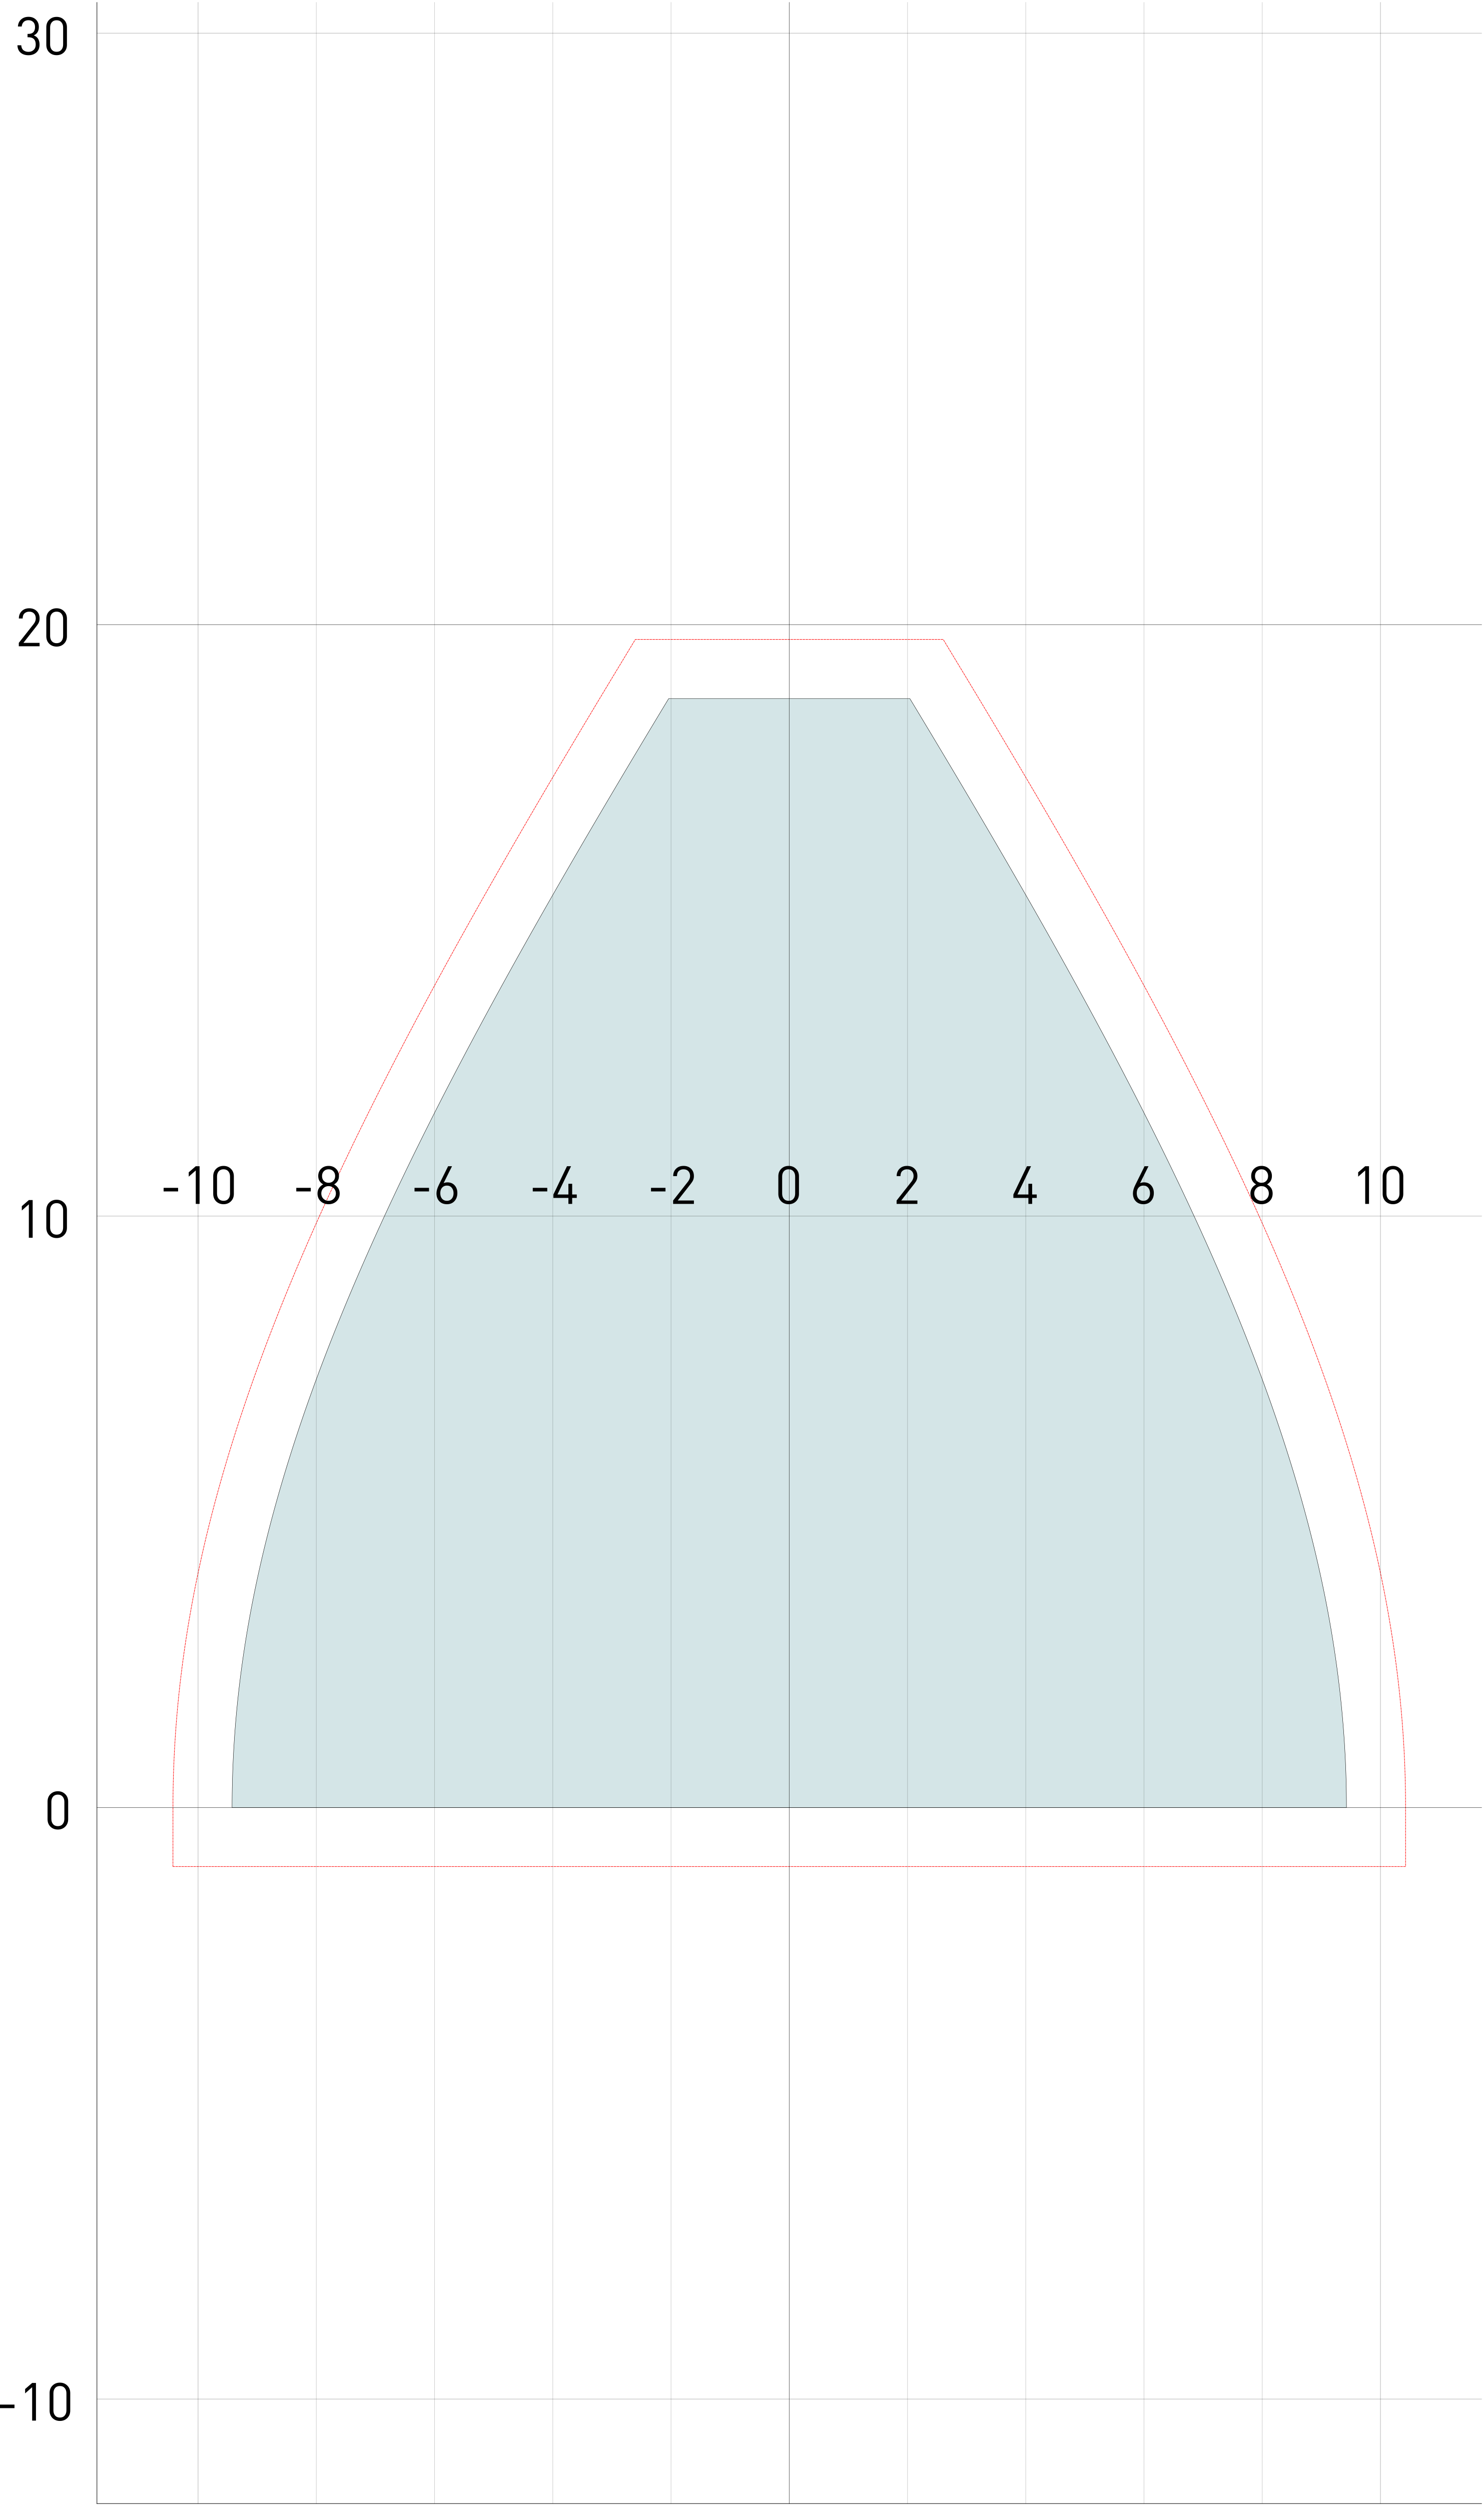
\includegraphics[width=5cm]{images/PlotItem_2.png}
    \end{minipage}
}
\coloredbox{LightCyan1!50}{DeepSkyBlue4}{DeepSkyBlue4}{
    \begin{minipage}{0.4\textwidth}
    The second parachute was designed for use during calm weather conditions and had a diameter of 26.7 cm and a surface area of 444.9 square centimeters, which is designed to slow down the descent speed to 6 meters per second. 
    
    This parachute was optimized for stable and predictable conditions and is intended to provide a gentle and controlled descent of the CanSat during calm weather conditions.
    \end{minipage}
    \hfill
    \begin{minipage}{0.4\textwidth}
    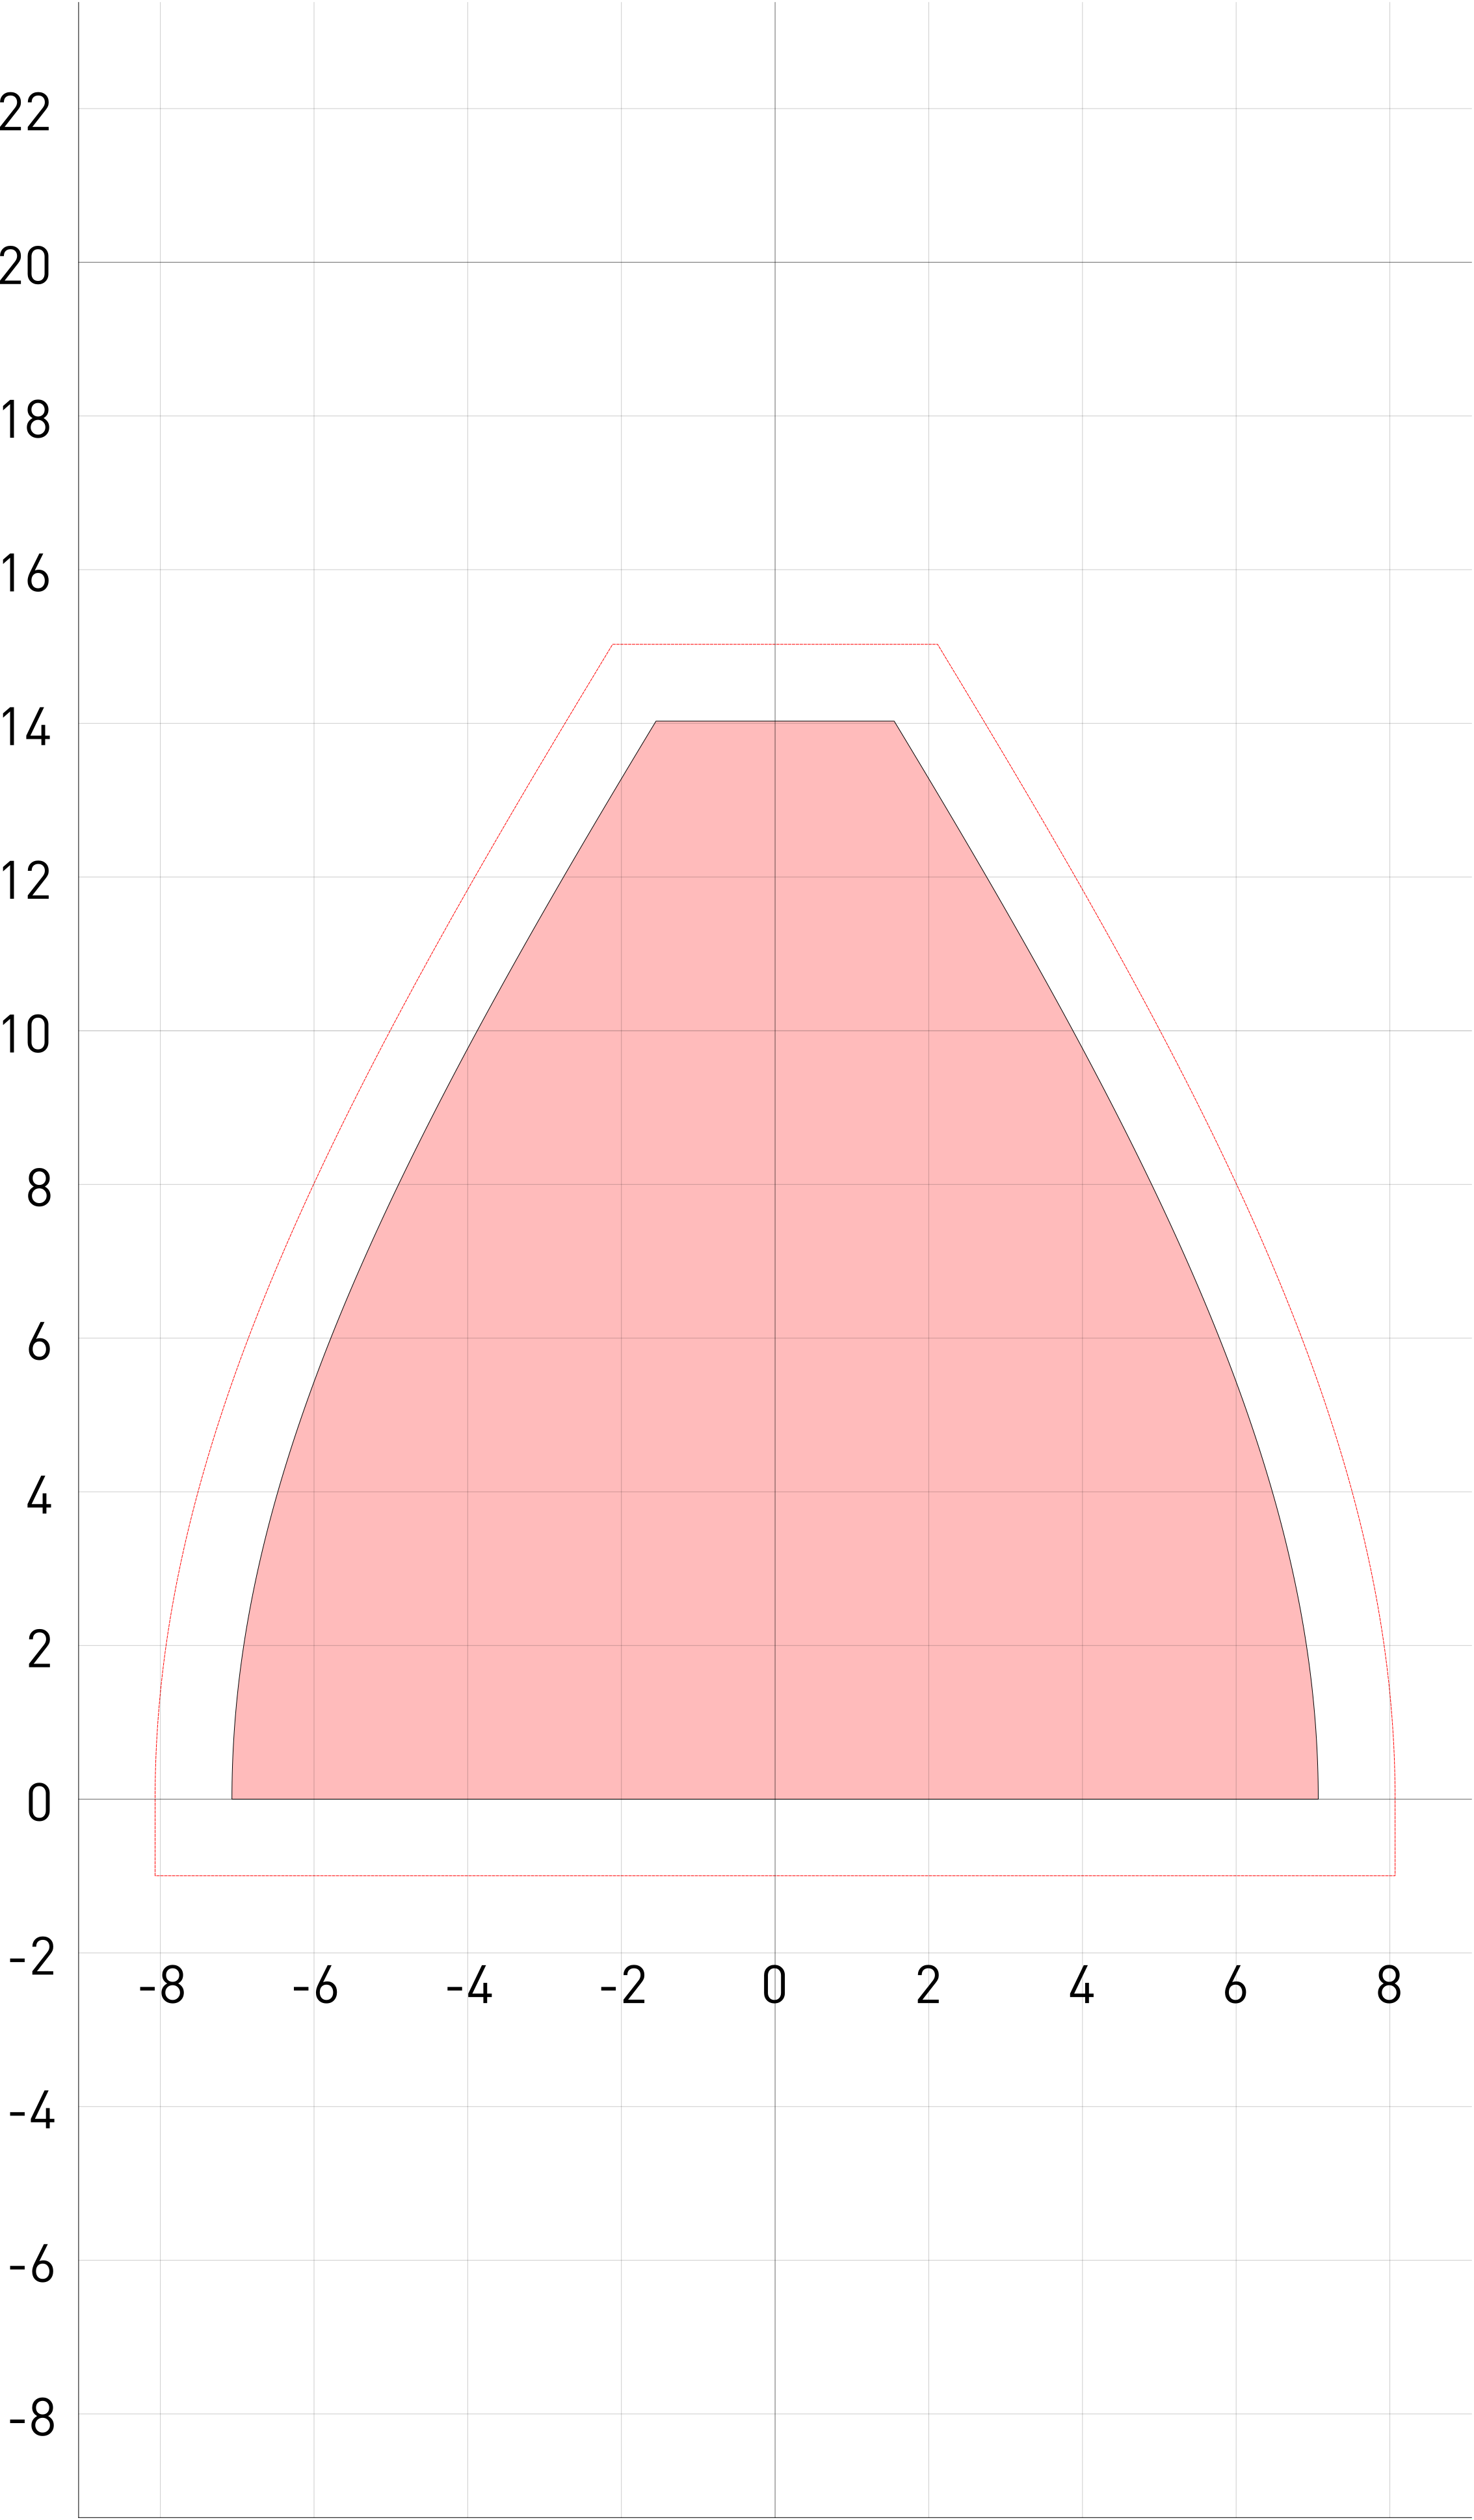
\includegraphics[width=5cm]{images/PlotItem_1.png}
    \end{minipage}
}

\subsubsection*{Ground Support Equipment}
\addcontentsline{toc}{subsubsection}{Ground Support Equipment}

In preparation for our upcoming mission, our team recognized the need to ensure that we have a reliable and efficient base station for our CanSat system. To achieve this, we decided to take a two-pronged approach to our base station development.

Firstly, we decided to reuse our old base station, which was based on LoPy from Pycom. This base station had been used in previous missions and had proven to be highly reliable and effective. We believed that this approach would provide us with a solid foundation for our base station system and ensure that we have a reliable backup in case of any unforeseen issues.

Secondly, we decided to design a new base station based on Raspberry Pico. This decision was based on our desire to explore new technologies and capabilities and to create a more advanced and sophisticated system that could meet our evolving needs. The Raspberry Pico offered us greater processing power, enhanced connectivity, and increased flexibility, which we believed would be instrumental in achieving our goals.

However, the progress of our new base station design has been put on hold due to delays in the delivery of our components from our manufacturer in China, JLCPCB. This has caused some frustration and has forced us to reassess our timelines and project schedules. However, we remain committed to this approach and believe that the benefits of the new base station design will outweigh the short-term setbacks we are currently experiencing.

\subsection*{Equipment testing}
\addcontentsline{toc}{subsection}{Equipment testing}


Our team has made significant progress in testing the prototyped CanSat and sensors individually. We have conducted several specific tests on the sensors to ensure that they are functioning correctly, including pressure sensor tests, temperature sensor tests, humidity sensor tests, UV sensor tests, and GPS tests.

For the pressure sensor test, we exposed the used sensor to a pressure change and compared the results with a reference device. We placed both sensors in a sealed container with a known volume of air and measured the pressure change with a manometer or a barometer. The test was considered positive when both sensors showed the same pressure without measuring errors.

Similarly, for the temperature sensor test, we checked whether the target device and the reference device showed the same temperature within 24 hours. We placed both sensors in the same location and monitored their temperature readings at regular intervals for 24 hours. The test was considered positive when both sensors showed the same temperature without significant deviation.

For the humidity sensor test, we placed the target sensor and the reference device in a humidity chamber where the humidity was increased or decreased to a specific level, and the readings were compared. The target sensor and the reference device were placed in a humidity chamber where the humidity level was gradually increased or decreased to a specific level. The readings from both sensors were recorded and compared. The test was considered positive when both sensors showed the same humidity level without significant deviation.

Additionally, for the UV sensor test, we exposed the target sensor and the reference device to UV radiation from a UV light source and compared the readings. The target sensor and the reference device were exposed to UV radiation from a UV light source for a specific duration, and the readings were recorded and compared. The test was considered positive when both sensors showed the same UV index without significant deviation.

Moreover, we conducted a GPS test to test the accuracy of the GPS module by comparing the location obtained by the CanSat with the actual location. We recorded the location data collected by the GPS module during this time and compared it to the actual location using a separate reference system.


\subsection*{Project planning}
\addcontentsline{toc}{subsection}{Project planning}

Our team is thrilled to report that we have made significant progress in the CanSat development process. We have successfully completed the initial prototyping phase, which allowed us to test the individual sensors and ensure that they are functioning correctly. In addition, we have conducted several rigorous tests on the CanSat's structure to verify its durability and endurance, and we are pleased to report that it has performed well under these challenging conditions.

With the necessary components and materials identified, we are now working tirelessly to integrate them into the final CanSat design. Our team is determined to deliver a high-quality product that meets our expectations and exceeds the competition requirements.

As we move forward, we recognize the importance of continuing our testing and refinement process to ensure that the CanSat performs to the best of its ability. To this end, we have scheduled the final PCB integration and testing phase for the last week before the launching campaign. This will allow us to thoroughly test the CanSat's electronics, ensuring that they are fully functional and performing optimally.




\section{Introduction}

\subsection{Purpose of the mission}

The primary goal of our CanSat mission is to carry out an extensive examination of a planet's environment, encompassing factors like air quality, lighting conditions, wind velocities, landscape classification, temperature, pressure, and aerial footage, to determine its suitability for life and evaluate the prerequisites for its support. The information obtained via our CanSat will be employed to gather crucial insights and formulate strategies for further planetary exploration. Our mission seeks to deliver essential data to the ground station about the environment investigated during a space mission.

\subsection{Team organisation and roles}

\subsubsection{Team name}
The team name {\textbf{CDOSR}} stands for Coderdojo Oradea Space Robotics, a group focused on space and robotics technologies, originating from CoderDojo Oradea. 

CoderDojo Oradea is a community-based programming club located in Oradea, Romania. It is part of the global CoderDojo network, which aims to provide free, volunteer-led coding sessions for young people between the ages of 7 and 17. The primary goal of CoderDojo Oradea is to inspire and encourage children and teenagers to learn to code, develop programming skills, and explore technology in a fun and supportive environment.

CDOSR (CoderDojo Oradea Space Robotics) is a specialized division within CoderDojo Oradea that focuses on space robotics and related technologies. This division brings together young enthusiasts who are passionate about space exploration and robotics, offering them a platform to learn, collaborate, and develop innovative solutions for real-world space-related challenges.

\subsubsection{Team composition}

The Space Robotics team of CoderDojo Oradea consists of a team leader and six members who are all between the ages of 14 and 18. Although they attend different high schools in Oradea, they are all members of the CoderDojo Oradea community. Some of the team members have previously participated in the national CanSat competition. The team has consistently been selected for the national finals for the past five years. The CoderDojo Club's activities are limited to Saturdays.

Each team member has a primary role that they diligently fulfill and secondary roles that allow them to learn from their teammates and promote collaboration within the team.

Our team structure emphasizes open communication, facilitating brainstorming and fostering creative problem-solving. This approach also aids in the decision-making process, as everyone is encouraged to seek help and assistance from other team members to ensure that any uncertainties are addressed.

\begin{itemize}
    \item[] \textbf{Daniel Erzse (teacher)}
    \begin{itemize}[label=\ding{109}]
        \item[\faCogs] \textbf{Previous Experience:} 
        \begin{itemize}[label=\ding{59}]
            \item Taught Advanced Mathematics, Statistics, and Astronomy as a university lecturer for over 17 years.
            \item Coordinates and mentors the local CoderDojo in Oradea for the last four years.
            \item Led CoderDojo teams in Astro Pi and CanSat competitions, as well as in the Exo-RO Rover Challenge.
        \end{itemize}
        \item[\faGraduationCap] \textbf{Background and Interests:} 
        \begin{itemize}[label=\ding{59}]
            \item STEM teacher with a passion for hands-on projects as the best way to teach and learn.
        \end{itemize}
        \item[\faMicroscope] \textbf{Field of Work (Role):} Team leader and software advisor. Coaching and coordinating the team.
        \item[\faLaptopCode] \textbf{Expected Workload:} 10 hours/week (3 hours/week at CoderDojo, 7 at home)
    \end{itemize}
    \vspace{0.2 cm}
    \item[] \textbf{Elisa Erzse}
    \begin{itemize}[label=\ding{109}]
        \item[\faCogs] \textbf{Previous Experience:} 
        \begin{itemize}[label=\ding{59}]
            \item Participated in the CanSat competition as a team member of CDOSR in 2022.
        \end{itemize}
        \item[\faGraduationCap] \textbf{Background and Interests:} 
        \begin{itemize}[label=\ding{59}]
            \item 11th-grade student at "Mihai Eminescu" National College, Oradea, Oradea.
            \item Passionate about IT and programming.
            \item Has been a member of CoderDojo Oradea since 2014.
            \item Joined the robotics group at CoderDojo Oradea three years ago at the age of 14 after the first participation of the group in CanSat.
        \end{itemize}
        \item[\faEdit] \textbf{Contribution:} Writing mission reports and data analysis, planning outreach programs, and presenting the mission to the judges. 3D modeling for the CanSat prototypes. Programming, technical design. PR \& social network tasks. Journalist. 
        \item[\faMicroscope] \textbf{Field of Work (Role):} Software design and high-level programming, Data analysis and interpretation, 3D modeling, and Social networking.
        \item[\faLaptopCode] \textbf{Expected Workload:} 7 hours/week (3 hours/week at CoderDojo, 4 at home).
    \end{itemize}
    \vspace{0.2 cm}
    \item[] \textbf{Kevin Caba}
    \begin{itemize}[label=\ding{109}]
        \item[\faCogs] \textbf{Previous Experience:} 
        \begin{itemize}[label=\ding{59}]
            \item Participated in Coolest Projects Romania and Coolest Projects Dublin in the Hardware section of the competition in 2017 and 2018.
            \item Participated in the CanSat and Exo-Ro competitions as a team member of CDOSR in 2021.
        \end{itemize}
        \item[\faGraduationCap] \textbf{Background and Interests:} 
        \begin{itemize}[label=\ding{59}]
            \item 11th-grade student, currently 17 years old.
            \item Passionate about Electronics and Programming since the age of 10.
            \item Has been part of the robotics group at CoderDojo Oradea since 2017.
        \end{itemize}
        \item[\faEdit] \textbf{Contribution:} Circuit/electrical design. Software design (GPS and GSM communication) and testing. He will work mainly on the communication interface with the CanSat and data analysis. Outreach programs and PR.
        \item[\faMicroscope] \textbf{Field of Work (Role):} Hardware design, Software design and high-level programming, Electronics \& software integration.
        \item[\faLaptopCode] \textbf{Expected Workload:} 7 hours/week (3 hours/week at CoderDojo, 4 at home).
    \end{itemize}
    \vspace{0.2 cm}
    \item[] \textbf{Alin Lup\u{a}u}
    \begin{itemize}[label=\ding{109}]
        \item[\faCogs] \textbf{Previous Experience:} 
        \begin{itemize}[label=\ding{59}]
            \item Participated in multiple projects for ESA's AstroPi program.
            \item Presented a robotics application at Coolest Projects International 2017 at the age of 8, along with his older brother Catalin.
        \end{itemize}
        \item[\faGraduationCap] \textbf{Background and Interests:} 
        \begin{itemize}[label=\ding{59}]
            \item 14-year-old high school student.
            \item Has a great interest in Physics, Astronomy, and Programming.
            \item Experienced in robotics and programming, having participated in the Coolest Projects International at a young age.
            \item Eager to learn and develop skills in areas related to science and technology.
        \end{itemize}
        \item[\faEdit] \textbf{Contribution:} 
        \item[\faMicroscope] \textbf{Field of Work (Role):} Team leader and software advisor. Coaching and coordinating the team.
        \item[\faLaptopCode] \textbf{Expected Workload:} 7 hours/week (3 hours/week at CoderDojo, 4 at home).
    \end{itemize}
    \vspace{0.2 cm}
    \item[] \textbf{Andrei Fazekas}
    \begin{itemize}[label=\ding{109}]
        \item[\faCogs] \textbf{Previous Experience:} 
        \begin{itemize}[label=\ding{59}]
            \item Assisted other teams at CDOSR to gain experience and knowledge.
        \end{itemize}
        \item[\faGraduationCap] \textbf{Background and Interests:} 
        \begin{itemize}[label=\ding{59}]
            \item 9th-grade student at "Don Orione" High School in Oradea.
            \item Has experience using Autodesk Fusion 360.
            \item Member of CoderDojo since 2018.
            \item Interested in developing skills related to programming and technology.
            \item Eager to contribute to the team's success by applying the skills and knowledge he has gained.
        \end{itemize}
        \item[\faEdit] \textbf{Contribution:} Assist with the design and prototyping of the CanSat using Autodesk Fusion 360. Modeling and developing 3D components of the CanSat.
        \item[\faMicroscope] \textbf{Field of Work (Role):} Hardware design, 3D modeling.
        \item[\faLaptopCode] \textbf{Expected Workload:} 7 hours/week (3 hours/week at CoderDojo, 4 at home).
    \end{itemize}
    \vspace{0.2 cm}
    \item[] \textbf{Vlad Marian}
    \begin{itemize}[label=\ding{109}]
        \item[\faCogs] \textbf{Previous Experience:} 
        \begin{itemize}[label=\ding{59}]
            \myitemtwo Has two years of membership in the FTC team, Modus Vivendi, at "Mihai Eminescu" National College.
        \end{itemize}
        \item[\faGraduationCap] \textbf{Background and Interests:} 
        \begin{itemize}[label=\ding{59}]
            \item 11th-grade student at "Mihai Eminescu" National College.
            \item  Joined the team one year ago and is dedicated to learning as much as he can about Computer Science and Robotics.
            \item  Believes that life is a continuous learning process and wants to seize each moment he can.
        \end{itemize}
        \item[\faEdit] \textbf{Contribution:} He will be responsible for programming and software design, specifically focusing on initial testing and concept design for the CanSat and ground station software. Additionally, he will work on developing the 3D modeling for the CanSat design.
        \item[\faMicroscope] \textbf{Field of Work (Role):} Software design and high-level programming, 3D modeling. Assistance in electronics integration.
        \item[\faLaptopCode] \textbf{Expected Workload:} 7 hours/week (2 hours/week at CoderDojo, 5 at home).
    \end{itemize}
    \vspace{0.2 cm}
    \item[] \textbf{Andrei Droj}
    \begin{itemize}[label=\ding{109}]
        \item[\faCogs] \textbf{Previous Experience:} 
        \begin{itemize}[label=\ding{59}]
            \item Former member of the winning team at ExoRo 2021.
            \item Team member in the CoderDojo Oradea and Modus Vivendi joint team, participating in the Qube2Space competition in 2022.
        \end{itemize}
        \item[\faGraduationCap] \textbf{Background and Interests:} 
        \begin{itemize}[label=\ding{59}]
            \item 11th-grade student at "Mihai Eminescu" National College, Oradea.
            \item Member of CoderDojo Oradea since 2015.
            \item Interested in embedded programming and hardware design.
            \item Considers competitions as a great opportunity to learn new things.
        \end{itemize}
        \item[\faEdit] \textbf{Contribution:} Serve as a base operator during the CanSat mission, monitoring and controlling the CanSat and ground station; assist with radio communications during the mission, ensuring clear and reliable communication between the CanSat and the ground station and assist with data analysis and interpretation, using software tools to analyze the data transmitted from the CanSat.
        \item[\faMicroscope] \textbf{Field of Work (Role):} Data analysis and interpretation,  Base operator, radio communications.
        \item[\faLaptopCode] \textbf{Expected Workload:} 7 hours/week (2 hours/week at CoderDojo, 5 at home).
    \end{itemize}
\end{itemize}

Our team is diverse and experienced, with members coming from robotics and 3D design competitions like ESA’s MoonCamp Project, CanSat, and First Tech Challenge. However, we understand that everyone can’t be assigned to their own specific subgroup. It is crucial for all team members to work closely together and share knowledge in order to help make the project a success. Collaboration and communication between team members are essential so that everyone can be involved in the project. By encouraging collaboration among team members, we can discuss issues as they arise and work to resolve them as effectively as possible.

\subsubsection{Team's Activity:} 

The team has developed a 7-point action plan to ensure effective progression in the CanSat design and development process, including:
\begin{enumerate}[topsep=3pt]
    \item Utilize the expertise and knowledge of each team member to collaborate on the project effectively:
    \begin{itemize}[leftmargin=0.25cm,itemindent=0.5cm, noitemsep, topsep=2pt, label=\ding{59}]
        \item Identify the strengths and areas of expertise of each team member.
        \item Encourage open communication and idea-sharing to facilitate collaboration.
        \item Create a team environment that values input and feedback from all members.
    \end{itemize}
    \item Establish a clear plan and timeline for the design, development, and testing phases of the CanSat:
    \begin{itemize}[leftmargin=0.25cm,itemindent=0.5cm, noitemsep, topsep=2pt, label=\ding{59}]
        \item Develop a detailed plan outlining specific milestones, deadlines, and deliverables for each phase of the project.
        \item Regularly review and update the plan to ensure it remains on track and adaptable to any changes or challenges that may arise.
    \end{itemize}
    \item Regularly communicate and meet to discuss progress, challenges, and potential solutions:
    \begin{itemize}[leftmargin=0.25cm,itemindent=0.5cm, noitemsep, topsep=2pt, label=\ding{59}]
        \item Schedule regular team meetings to discuss progress and challenges.
        \item Provide updates on individual tasks and responsibilities to ensure the team is working efficiently and effectively.
        \item Encourage open communication and idea-sharing to facilitate collaboration and problem-solving.
    \end{itemize}
    \item Allocate specific roles and responsibilities to each team member based on their skills and interests:
    \begin{itemize}[leftmargin=0.25cm,itemindent=0.5cm, noitemsep, topsep=2pt, label=\ding{59}]
        \item Identify each team member's strengths and areas of expertise.
        \item Allocate roles and responsibilities based on these strengths and interests.
        \item Ensure each team member has a clear understanding of their role and responsibility in the project.
    \end{itemize}
    \item Utilize various resources, including online resources and tools, to support the team's progress and development:
    \begin{itemize}[leftmargin=0.25cm,itemindent=0.5cm, noitemsep, topsep=2pt, label=\ding{59}]
        \item Research and utilize various online resources and tools to support the design and development process.
        \item Keep up to date with relevant news, updates, and industry trends to enhance the team's knowledge and expertise.
    \end{itemize}
    \item Continuously test and evaluate the CanSat design to ensure it meets competition requirements and performs as expected:
    \begin{itemize}[leftmargin=0.25cm,itemindent=0.5cm, noitemsep, topsep=2pt, label=\ding{59}]
        \item Develop a testing plan to ensure the CanSat design meets competition requirements and functions as expected.
        \item Regularly evaluate the design to identify areas for improvement and potential issues.
        \item Continuously iterate and improve the design based on feedback and testing results.
    \end{itemize}
    \item Seek feedback and input from mentors and advisors to enhance the design and development process:
    \begin{itemize}[leftmargin=0.25cm,itemindent=0.5cm, noitemsep, topsep=2pt, label=\ding{59}]
        \item Regularly seek feedback and input from mentors and advisors to enhance the design and development process.
        \item Utilize feedback and input to improve the design and development process and enhance the team's knowledge and expertise.
    \end{itemize}
\end{enumerate}


\subsection{Mission objectives}

{\textit{“Make life multiplanetary” - Elon Musk}}
\vspace{0.5cm}

The mission objective for the CanSat team is to conduct an atmospheric and landing site survey at an altitude of roughly 1000 meters. This survey aims to determine the feasibility of future missions for more in-depth exploration. During the flight, the CanSat will have two missions: one primary and one secondary.

During its flight, the CanSat will take pictures using the mounted camera to capture the terrain during the descent. The team plans to categorize the terrain in the photographs to gain a better understanding of the surrounding landscape. Additionally, the CanSat will continuously collect and send important data such as position, temperature, pressure, humidity, and UV index throughout its flight.

\subsubsection{Missions description}

The CanSat's \textbf{primary mission}, following its release and during its descent, is to measure air \textbf{temperature} and air \textbf{pressure}. It will transmit this data to the ground station at least once every second. The data collected will be analyzed using the barometric formula to determine the CanSat's altitude.

The secondary mission of the CoderDojo Space Robotics project extends beyond its primary objectives by measuring additional parameters, such as humidity, UV light, carbon dioxide, and particulate matter (PM), in addition to telemetry data, incorporating the following tasks:
\begin{itemize}[leftmargin=1.27cm, itemindent=0cm, topsep=2pt, label=\faTasks]
    \item {\textbf{Atmospheric Science:}} The CanSat will measure and record atmospheric data at different altitudes, such as temperature, humidity, and pressure. The data collected will be used to study the atmosphere and create a visual representation of the atmospheric profile.
    \item {\textbf{UV Radiation Detection:}} The CanSat will detect and record the amount of UV radiation at different altitudes during its descent. This data will be used to create a profile of the UV radiation intensity along the descending path. This information will help identify areas with high levels of UV radiation and raise awareness of the risks of skin damage and other health problems.
    \item {\textbf{Air Pollution:}} The CanSat will measure and record air quality data at different altitudes, such as carbon monoxide and ozone levels. This data will be analyzed to identify sources of pollution and inform public policy decisions related to air quality.
    \item {\textbf{Mapping:}} The CanSat will be equipped with cameras and other sensors to collect data on land features from high altitudes. This information will be used to create detailed maps of the area.
\end{itemize}
\subsubsection{Measurements, investigations and tests}

We will collect geolocation data that will be analyzed to determine the precise location of the CanSat and to create a map of the surrounding area. This information can be used to identify potential landing sites for future missions and to gain a better understanding of the environment. 

The CanSat software aims to create topographic maps using photographs taken during the mission. The application starts immediately after the launch and captures images, which will be classified by a convolutional neural network (CNN) to obtain terrain classifications. CNN is a type of neural network that uses special filters to reduce the number of parameters required to train the model. The development of the ML classifier and the transmission and reception of data are both major objectives of the mission and significant effort will be dedicated to their development.

Real-time transmission will be implemented for some of the measured data using a LoraWAN network, while the remaining data collected at a higher frequency will be stored on a flash memory and microSD card for post-retrieval analysis, if the recovery is possible. The sensor and camera data will be analyzed to reconstruct the descent trajectory and generate topographic representations of the surrounding environment during the descent phase.

To transform the collected data into a meaningful story, our team recognizes the importance of data analysis. We understand that this analysis is a crucial step after data collection from the satellite, and we will ensure that the information obtained is utilized effectively. We plan to use various methods to analyze the data collected from the CanSat. Depending on the data type, different tools will be required for analysis. The methods we will employ for analyzing sensor data include visual representation using charts and graphs, generation of tables for variable comparison, and performing calculations on numerical data.

Indeed, gathering atmospheric data for the CDOSR project is not only crucial for environmental reasons, but also for technical reasons. The CanSat will operate in a challenging and dynamic environment, with rapidly changing atmospheric conditions, such as temperature, humidity, and pressure.

Therefore, there are several additional reasons why the CDOSR team may have selected the secondary mission of measuring atmospheric data and air pollution at different altitudes.

One reason is to test new materials for the parachute, which is a critical component of the CanSat's descent system. The team may be using an extremely lightweight Cordura nylon material for the parachute to increase its effectiveness while reducing the satellite's overall weight. By measuring atmospheric data during the descent, the team can evaluate the parachute's performance and determine whether the new material is suitable for future missions.

Another reason may be to test a new microcontroller for the main board, which is responsible for controlling and coordinating the various systems on the CanSat. Gathering atmospheric data during the mission can help the team evaluate the microcontroller's performance in real-world conditions and identify any areas for improvement.

Moreover, the team may be exploring the feasibility of using a modular design for different types of sensors. By gathering atmospheric data and air pollution data, the team can evaluate the performance of various sensors and determine which ones are best suited for future missions. Additionally, the team may be exploring the possibility of using one microcontroller core to process images during the descent, which can reduce the weight and complexity of the CanSat's onboard systems.

\subsubsection{Research expectations}

The CDOSR team expects to gain several insights and knowledge from the secondary mission of measuring atmospheric data and air pollution at different altitudes.

The team's primary objective is to gain a better understanding of the atmospheric conditions and their impact on the CanSat's performance and operation. By precisely measuring various parameters such as temperature, humidity, and pressure at different altitudes, the team aims to optimize the design and operation of the CanSat's systems, ensuring its survival and successful mission completion.

As the altitude increases, the atmospheric conditions undergo significant changes. The team expects a decrease in temperature of around 6.5 °C per kilometer, which is approximately the value of the vertical thermal gradient in the troposphere under standard conditions\endnote{
    {\href{https://en.wikipedia.org/wiki/Atmospheric\_temperature\#Temperature\_versus\_altitude}
    {https://en.wikipedia.org/wiki/Atmospheric\_temperature}}}. Moreover, using both linear and exponential Stevin's law\endnote{
    {\href{https://en.wikipedia.org/wiki/Vertical\_pressure\_variation}
    {https://en.wikipedia.org/wiki/Vertical\_pressure\_variation}}}, 
the team should detect a decrease in air pressure of approximately 120 hPa per 1000 meters. As a consequence, there should be also a slight decrease in relative humidity since it is directly proportional to the air pressure. These insights will help the team to design and optimize the CanSat's systems to withstand the changing atmospheric conditions during the mission.

Secondly, the team hopes to gain insights into the levels of UV radiation and air pollution at different altitudes. By collecting and analyzing this data, the team can identify sources of pollution and raise awareness of the risks of skin damage and other health problems associated with high levels of UV radiation.

Moreover, the team hopes to gain insights into the data collection, transmission, and analysis process for future space-related projects. By equipping the CanSat with cameras and other sensors, the team can collect data on land features from high altitudes and create detailed maps of the area. This can inform urban planning, disaster management, and other applications.

Overall, the CoderDojo Space Robotics project team expects to gain valuable insights and knowledge from the secondary mission of measuring atmospheric data and air pollution at different altitudes, contributing to the broader goal of promoting environmental sustainability and advancing space-related technology.

\subsubsection{Objectives for a successful mission}

The below objectives are to be achieved on launch day and post-launch analysis:
\begin{multicols}{2}[\vspace{-0.75\baselineskip}]
\begin{itemize}[leftmargin=1cm,itemindent=0.5cm, noitemsep, topsep=2pt, label=\ding{51}]
    \item Successful launch
    \item Live data transmission and  telemetry
    \item GSM Data
    \item Successful parachute deploy
    \item All systems nominal (reliable sensor and location data)
    \item Descent rate between 5-10 \SI{}{\meter\per\second}
    \item Landing confirmation
    \item Recovery of the can
    \item AI data analysis
    \item Generating reports
\end{itemize}
\end{multicols}

In conclusion, the primary mission of the CanSat project is to measure and transmit atmospheric data such as temperature, pressure, and altitude, while the secondary mission includes additional measurements such as humidity, UV radiation, air pollution, and telemetry data. 

The importance of gathering atmospheric data for space-related projects cannot be overstated, as it provides crucial insights into the environmental conditions in which the project operates, optimizes its design, and contributes to broader sustainability efforts.

Understanding the atmospheric conditions is essential for the successful operation of any space-related project. The atmosphere plays a crucial role in determining the behavior of a satellite, such as its trajectory and orientation. Temperature, pressure, and humidity can affect the functioning of onboard electronics, while exposure to high levels of UV radiation can damage the satellite's surface and components.

By gathering atmospheric data at different altitudes, the team can gain a comprehensive understanding of the environment in which the CanSat will operate. This information can be used to optimize the satellite's design and operating procedures, ensuring its survival and successful completion of the mission. Moreover, the data collected can be compared with existing models of the Earth's atmosphere to improve their accuracy and reliability.

\section{CanSat description}

\subsection{Mission Overview}

The CoderDojo Space Robotics project team will execute the mission by designing and constructing a CanSat that will launch and deploy from a rocket at an altitude of approximately 1000 meters. During the CanSat's descent, it must maintain a speed between 5 and 10 meters per second, while collecting and transmitting data on various environmental parameters, including temperature, pressure, space positioning, location, image data, UV radiation, different types of gases (pollution), and the concentration of particulate matter. All of this data will be transmitted in real-time to the ground station and stored onboard. After landing, the CanSat will signal its coordinates using a buzzer and a light beacon, activating the recovery system.

These key elements will play an essential role in accomplishing the mission objectives. Here is a brief explanation of each element:
\begin{itemize}[leftmargin=1.27cm, itemindent=0cm, topsep=2pt, label=\faTasks]
    \item[\faThermometerQuarter] \textbf{Sensor System}: A sensor system is critical to the mission's success as it helps to measure various parameters that are important for the experiment. The sensor system can measure parameters such as temperature, pressure, inertial performance, UV, light intensity, and particulate matter. These measurements will provide valuable data for the post-launch data analysis.
    \coloredbox{LightCyan1!50}{DeepSkyBlue4}{DeepSkyBlue4}{
        {During the descent, the CanSat will record, store, and transmit the following data:
        \begin{multicols}{2}[\vspace{-0.6\baselineskip}]
            \begin{itemize}[noitemsep, topsep=0pt, label=\ding{111}]
                \item Humidity and air temperature
                \item Barometric pressure
                \item GPS Location
                \item Magnetic field
                \item Orientation
                \item Position in space using a gyroscope
                \item UV Index
            \end{itemize}
        \end{multicols}
        \vspace*{-0.75\baselineskip}
        }
    }
    \item[\faMicrochip] \textbf{ESP32 Microcontroller}: The ESP32 microcontroller is responsible for controlling the various subsystems of the CanSat. It provides a reliable and efficient way to control the CanSat's functions, making it a crucial part of the overall system.
    \item[\faBroadcastTower] \textbf{Telemetry Syste}m: The telemetry system is responsible for sending data back to the ground station. It uses GSM and RF modules to transmit data, which can be analyzed in real time by the mission team. This system helps to ensure that the mission objectives are met and that the data collected is of high quality.
    \item[ \faParachuteBox] \textbf{Recovery System}: The recovery system is essential to ensure the CanSat is safely returned to the ground. It consists of visual and audible alarms that alert the ground station to the CanSat's location. This system will help to prevent damage to the CanSat and ensure that the data collected during the mission is preserved.
    \item[\faChartBar] \textbf{Post-Launch Data Analysis}: Post-launch data analysis is essential for interpreting the data collected during the mission. It allows the mission team to evaluate the success of the mission and determine whether the mission objectives were met. This analysis can help to inform future missions and experiments. 
\end{itemize}

%\begin{figure}[htbp]
%  \centering
%  \includesvg{img_Block_Diagram_2023.svg}
%  \caption{svg image}
%\end{figure}

\begin{figure}[htbp]
\centering
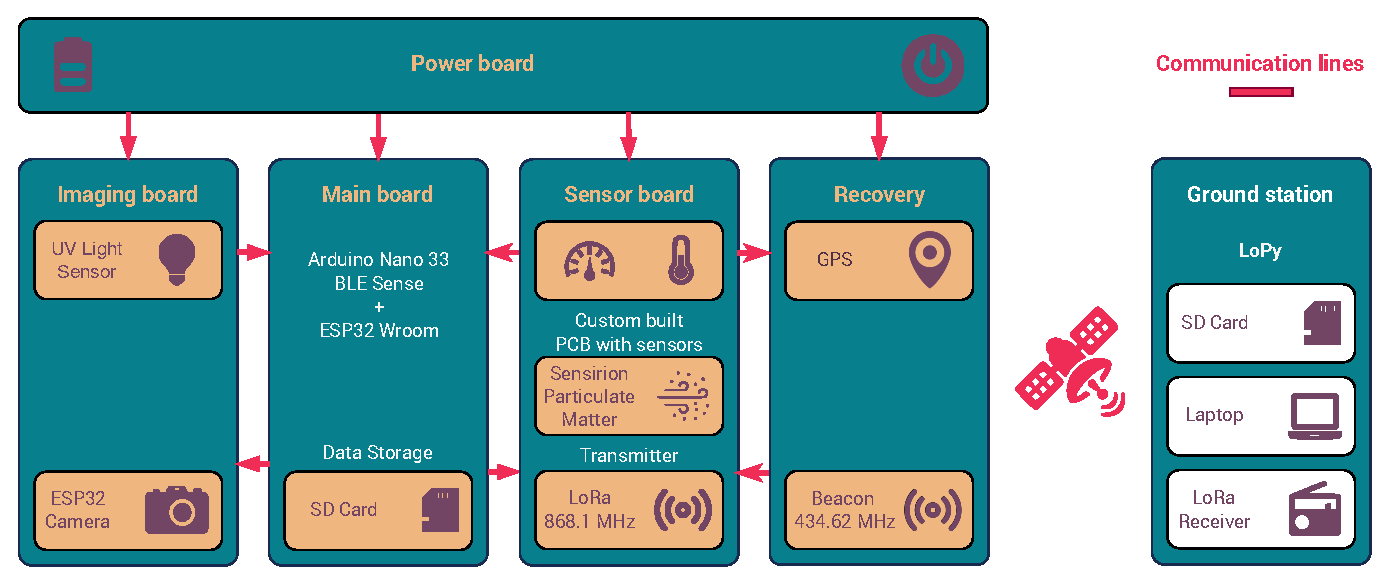
\includegraphics[width=\linewidth]{img_Block_Diagram_2023.eps}
\caption{\small{Base block diagram for the CanSat and the ground station.}}
\label{fig:bloc_diagrame}
\end{figure}

Several onboard devices will make the mission possible, the key ones being:
    \begin{multicols}{2}[\vspace{-0.5\baselineskip}]
        \begin{itemize}[leftmargin=1.75cm,itemindent=0cm, noitemsep, topsep=2pt, label=\faCheck]
            \item[\faMicrochip] MicroController (ESP32 Wroom with or without Arduino Nano 33 BLE Sense Board)
            \item[\faCamera] Cameras (ESP32 With Camera Module OV2640)
            \item[ \faWifi] Data transceiver (RN2483)
            \item[\faThermometerQuarter] Humidity and temperature sensors (BME 688, MCP 9808)
            \item[\faMapMarked] GPS (NEO-M8, L76GNSS)
            \item[\faCompass] Navigation sensor (LSM6DS33 gyroscope \& LIS3MDL compass )
            \item[\faBatteryHalf] High-performance batteries
            \item[\faCloudversify] Particulate Sensor (SPS30)
            \item[\newaltitudeicon] Altimeter (LPS25H)
            \item[\newgsmicon] GSM module (SIM800L)
        \end{itemize}
        \vspace*{-0.75\baselineskip}
    \end{multicols}

The ESP32 and Arduino Nano 33 BLE Sense boards are designed to collect data from various sensors during the flight, including location, temperature, and pressure. This data is stored on an SD card for later analysis, but it is also transmitted to the base station in real-time using the LoRa protocol.

In addition to collecting data from sensors, the boards also receive data from two GPS modules. This data is routed to the GSM communication module, which sends the GPS coordinates of the CanSat to the base station. This allows the mission team to track the CanSat's location and monitor its progress during the flight.

Overall, the combination of the ESP32 and Arduino Nano 33 BLE Sense boards provides a reliable and efficient way to collect and transmit data during the CanSat's flight. The data collected can be analyzed after the mission to gain insights into various environmental factors and improve future missions.


\subsection{Mechanical/structural design}

For the mechanical design, several factors have been considered to ensure the CanSat's robustness and easy maintenance:
\begin{itemize}[leftmargin=1.75cm,itemindent=0cm, noitemsep, topsep=3pt,  label=\faCheck]
    \item \textbf{Component protection}: The CanSat's structure has been designed to protect the components from any external impact or shock during the launch and landing;
    \item \textbf{Resilient structure}: The CanSat's structure includes shock-absorbing systems such as foam or gel-based layers, springs, or a combination of both. These systems will help to reduce the impact force during landing, preventing damage to the CanSat and its components.;
    \item \textbf{Easy removal of batteries and radio transmitters}: The batteries and radio transmitters are positioned in a way that allows for easy removal in case of any malfunction or for recharging and testing purposes.;
    \item \textbf{Easy access to components}: The CanSat's body has been designed to allow easy extraction of the components for maintenance or replacement in case of malfunctions
    \item \textbf{Easy removal of batteries and radio transmitter}s: The batteries and radio transmitters are positioned in a way that allows for easy removal in case of any malfunction or for recharging and testing purposes.
\end{itemize}

By taking these factors into account, the team aims to create a robust and reliable CanSat that can withstand the harsh conditions of the mission and deliver accurate data.

The CanSat's structure is made from a combination of Polylactic Acid (PLA) and Acrylonitrile Butadiene Styrene (ABS), two lightweight 3D printing materials that provide strength, durability, and exceptional design. This composition allows the can to withstand the stress of launch and landing while maintaining an aerodynamic shape. Additionally, the can is designed with a removable bottom section, providing easy access to its internal components. This allows for easy maintenance and repair of the can, without having to dismantle the entire structure.

Despite PLA's relatively low impact strength, the electronic components housed within the CanSat are protected by 3D-printed supports and foam. The high tensile strength of PLA, which is about 50 MPa, ensures that the 3D-printed parts remain intact when the parachute deploys, preventing disintegration.

The design of the can is also important to ensure its durability during the launch and landing process. It must withstand high levels of stress and force during these events, so the structure must be designed to distribute and absorb these forces. The can's aerodynamic design is also important for reducing air resistance and achieving maximum altitude during launch.

\begin{table}[htbp]
\centering
\arrayrulecolor{DeepSkyBlue4} % set color of vertical lines
\begin{tabular}{>{\centering\arraybackslash}m{1cm}>{\centering\arraybackslash}lc}
\hline
\rowcolor{DeepSkyBlue4}
&\textbf{\color{white!50}{CanSat Characteristics (description)}} & \textbf{\color{white}{Figure (units)}} \\
\hline
%\rowcolors{2}{LightCyan!50}{}
\adjustbox{valign=m}{
\includegraphics[width=0.6cm]{icons/weight.png}} & Total weight of the CanSat & 350 g \\
\rowcolor{LightCyan1!50}\adjustbox{valign=m}{
\includegraphics[width=0.5cm]{icons/diameter.png}} & Diameter of the CanSat & 66 mm\\
\adjustbox{valign=m}{
\includegraphics[width=0.5cm]{icons/recovery.png}} & Length of the recovery system,
including parachute & Max. 60 cm\\
\rowcolor{LightCyan1!50}
\adjustbox{valign=m}{
\includegraphics[width=0.6cm]{icons/time.png}} & Flight time scheduled & 2 min 45 s \\
\adjustbox{valign=m}{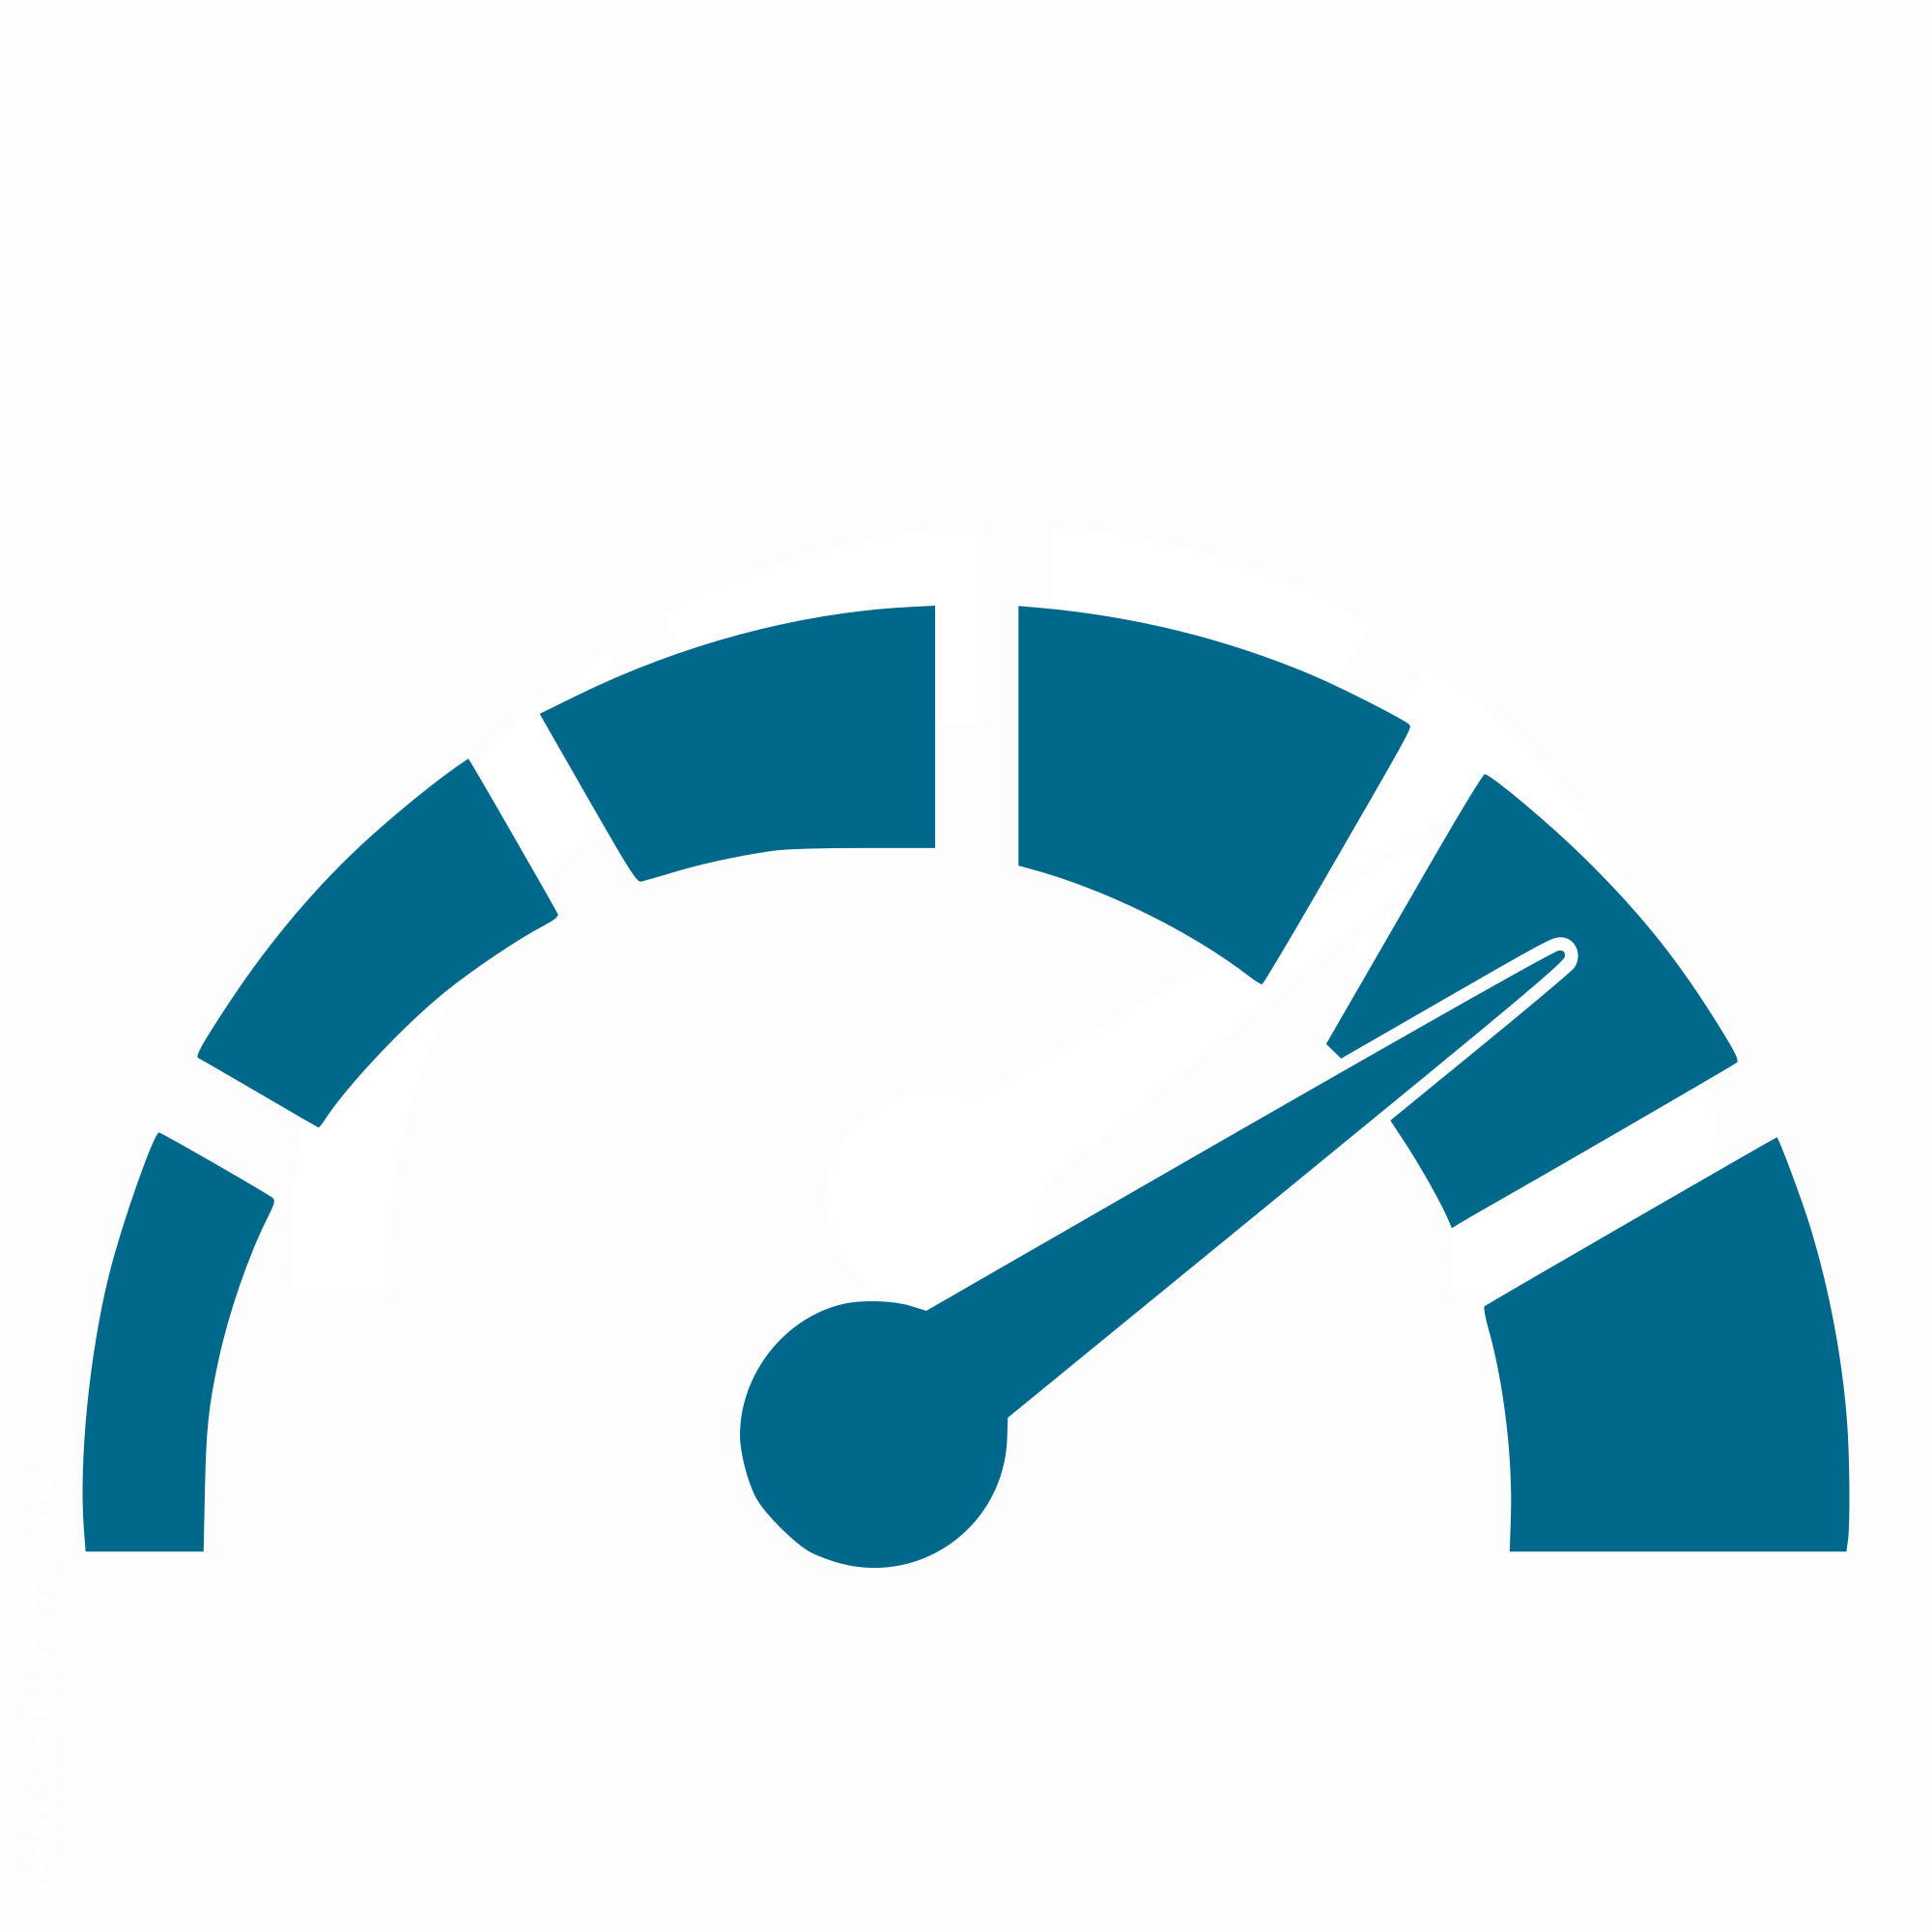
\includegraphics[width=0.6cm]{icons/descent-rate.png}} & Calculated descent rate of the CanSat & \SI{6 }{\meter\per\second} \\
\rowcolor{LightCyan1!50}
\adjustbox{valign=m}{
\includegraphics[width=0.6cm]{icons/frequency.png}} & Radiofrequency used for
communication & 868.1 MHz (LoRa) \\
\rowcolor{LightCyan1!50}
& & 434.42 MHz (beacon)\\
\adjustbox{valign=m}{
\includegraphics[width=0.5cm]{icons/power.png}} & Power consumption of the CanSat & 450 mA \\
\hline
\end{tabular}
\caption{\small{CanSat main characteristics}}
\end{table}

The CanSat is composed of several major components, including four PCB boards that house all the necessary modules. The battery pack, which is the largest and heaviest component, is located at the bottom of the can and contains two 18650 battery modules placed in a vertical position. The camera module is situated in the bottom middle of the can, along with a Sensirion SPS-30 particulate matter dust sensor. The upper part of the can houses the PCB layers, interconnected with mezzanine connectors, which are fixed in place using screws and glue. Despite the relatively heavy weight of the battery pack, the can is designed to withstand the stress of launch and landing, and the components are secured in place with 3D-printed supports and foam to prevent damage.

In order to ensure the functionality of the CanSat system during multiple tests, mechanical solutions were explored to protect the can and its contents from the impact of landing. After analyzing various options for shock-absorbing systems, we settled on prototyping and testing the most promising ideas based on their effectiveness, feasibility, and cost. Three potential concepts were identified, including:
\begin{itemize}[leftmargin=1cm,itemindent=0.5cm, noitemsep, topsep=0pt, label=$\bullet$]
    \item a foam or gel-based system;
    \item a spring-based system;
    \item a combined system using both foam or gel materials and springs.
\end{itemize}

The foam or gel-based system involves placing a layer of shock-absorbing foam or gel between two layers of the can, positioned at the bottom opposite to where the parachute is fastened. The spring-based system used a set of springs placed between two bottom layers of the can to compress and absorb the impact of the landing. Finally, the combined system used both springs and foam or gel materials to absorb the initial impact and further reduce the force of the landing, ultimately protecting the CanSat from damage.

The CanSat case is equipped with inserts along the inside to enhance its structural integrity. The lid is firmly secured using screws inserted into dedicated holes in the cap, ensuring that it cannot be opened without a screwdriver. Additionally, the case features strategically placed holes to allow for optimal camera positioning and airflow inside the can. 


\subsection{Electrical design}

The electrical design of our CanSat relies on the use of custom-made PCBs due to the limited space available in its interior. We have developed custom PCBs designed using Autodesk's EAGLE software to ensure that all the necessary components fit properly. 

Using custom PCBs provides several advantages for the CanSat project. Firstly, it allows for a better fit of all the components in the limited space available. This can increase the overall efficiency of the CanSat by reducing the size and weight of the PCBs while still accommodating all the necessary components. Secondly, custom PCBs can also help to reduce the risk of damage to the components during the launch and landing phases of the mission. By integrating the components into the PCB design, they are better protected from shocks and vibrations. Finally, designing custom PCBs allows for greater flexibility and customization in the CanSat's design, making it possible to optimize its performance and tailor it to specific mission requirements.

\subsubsection{Electrical Interface}
The electrical interface of the CanSat is designed to ensure a robust and reliable connection between its various electronic components. The main board serves as the central hub for the electrical interface, providing power and data connections to the sensors, transmitter, and other components.
\begin{figure}[htbp]
\centering
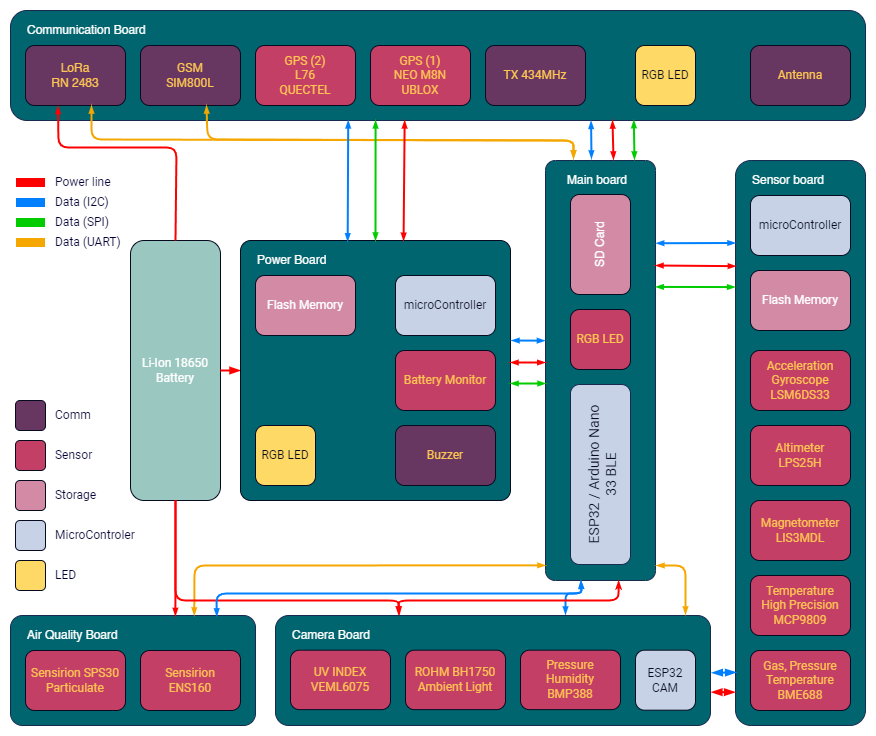
\includegraphics[width=\linewidth]{images/img_module_diagram.png}
\caption{\small{The Cansat block diagram with power and data lines.}}
\label{figmodule_diagrame}
\end{figure}

A small form factor size was chosen for the CanSat's mainboard and base station, consisting of an ESP32 Wroom module and an Arduino Nano 33 BLE Sense board. These components provide the necessary computing power and wireless communication capabilities for the mission. To ensure compatibility and flexibility, multiple types of connections were implemented between the microprocessor and other parts, such as UART, I2C, SPI, Digital Inputs, and Outputs.

An ESP32 module with a camera is used for the video recording and streaming feature of the CanSat. This camera is separated from the rest of the CanSat and is powered by the Power board, a custom-designed PCB. The ESP32 camera and the main microcontroller (which is an ESP32, backed by an Arduino Nano 33) are also powered by the Power board. The sensors for environmental parameter measurement, such as atmospheric pressure, temperature, and humidity, are placed on the same PCB as the ESP32 to reduce data line connectivity through the use of I2C connections. All data collected by the sensors are logged on an SD card and flash memory and are transmitted to the base station.

\begin{table}[htbp]
\centering
\arrayrulecolor{DeepSkyBlue4}
\begin{tabularx}{0.95\textwidth}{>{\raggedright\arraybackslash}p{3.5cm}c>{\raggedright\arraybackslash}X>{\raggedright\arraybackslash}p{5.5cm}}
\hline
\rowcolor{DeepSkyBlue4}
\textbf{\color{white!50}{Component}} & \textbf{\color{white!50}{Voltage}} & \textbf{\color{white!50}\textbf{Protocol}} & \textbf{\color{white!50}\textbf{Other Information}} \\ \hline
\rowcolors{2}{red}{}
ESP32-S3-Wroom & \SI{3.3}{\volt} & I2C, I2S, SPI, PWM, UART, USB & {Dual-core $\mu$Processor}\\ %\hline
\rowcolor{LightCyan1!50}ESP32 Cam Board & \SI{3.3}{\volt} & I2C, SPI, PWM, UART & {Dual-core $\mu$Processor}\\ %$\hline
Arduino Nano 33 BLE Sense & \SI{3.3}{\volt} & I2C, SPI, PWM, UART & {$\mu$Processor}\\ %\hline
\rowcolor{LightCyan1!50}AltIMU-10 v5 & \SI{3.3}{\volt} & I2C & Gyro, Accelerometer, Compass, and Altimeter\\ %\hline
MPU-6050 & \SI{3.3}{\volt} & I2C & MEMS Module, 3-Axis Gyroscope\/ Accelerometer\\ %\hline
\rowcolor{LightCyan1!50}BME688 & \SI{3.3}{\volt} & I2C & Air Quality Sensor, Humidity, Pressure \& Temperature Sensor\\ %\hline
BME280 & \SI{3.3}{\volt} & I2C & Humidity \& Pressure Sensor\\ %\hline
\rowcolor{LightCyan1!50}MCP9808 & \SI{3.3}{\volt} & I2C & Temperature Sensor\\ %\hline
VEML6075 & \SI{3.3}{\volt} & I2C & Photo IC Sensor\\ %\hline
\rowcolor{LightCyan1!50}VEML7700 & \SI{3.3}{\volt} & I2C & Ambient Light Sensor\\ %\hline
GUVA-S-12-D & \SI{3.3}{\volt} & ADC & UV Sensor\\ %\hline
\rowcolor{LightCyan1!50}SPS30 & 5V & I2C & Air Quality Sensors Particulate Matter \\ %\hline
SCD40 & 5V & I2C & Air Quality \& CO2 Sensor\\ %\hline
\rowcolor{LightCyan1!50}NEO-M9N & 5V & UART, SPI & GNSS / GPS Module\\ %\hline
Quectel L76 & \SI{3.3}{\volt} & UART, I2C & GNSS / GPS Module\\ %\hline
\rowcolor{LightCyan1!50}micro SD & \SI{3.3}{\volt} & SPI & Memory Card Connector\\ %\hline
64Mb Flash Memory & \SI{3.3}{\volt} & SPI & Flash Memory module \\ %\hline
\rowcolor{LightCyan1!50}SIM-800 & \SI{5}{\volt} & UART & GPRS GSM Module \\ %\hline
RN2483 LoRa Module& \SI{3.3}{\volt} & UART & Lora Modulation, \SI{868}{\mega\hertz} \\ %\hline
\rowcolor{LightCyan1!50}Power Switching Regulators & \SI{3.3}{\volt} & & High Efficiency Buck-Boost Converter  \\ %\hline
%U.FL-R-SMT Coaxial Connector & & & Antenna connector, 50$\Omega$ \\ \hline
\end{tabularx}
\caption{\small{Electronics Component Information}}
\end{table}

The ESP32 and Arduino Nano 33 microcontrollers are powered by the 3.3 Volt line from the power board, while certain components, such as the GSM module, require a higher 5 Volt line. The voltage range of the 18650-battery pack used to power the CanSat is within a safe range of 3.6V - 4.2V. To ensure that the batteries are used within this safe range, two buck-boost converters are employed to step down the voltage to 3.3V and up to 5V. These converters are capable of delivering up to 2A of continuous current, which provides enough power to run all the CanSat components without any risk of damaging them.

We can estimate the time that the CanSat can be powered using the following formula:

\begin{equation*}
\text{Time} = \frac{\text{Battery capacity} * \text{Voltage}}{\text{Power consumption}}=\frac{\SI{6800}{\milli\ampere} * \SI{4.2}{\volt}}{\SI{15.2}{\watt}} = \SI{1}{\hour}52\text{min}
\end{equation*}

The duration of 1 hour and 52 minutes is applicable when the CanSat's electronics operate at full capacity. However, since SMS messages are transmitted only twice per minute and some sensors go offline after landing, this operational time significantly extends to well over 3 hours.

\begin{table}[htbp]
\centering
\arrayrulecolor{DeepSkyBlue4}
\begin{tabular}{>{\raggedright\arraybackslash}p{4.9cm}c>{\raggedleft\arraybackslash}p{1.85cm}
>{\raggedleft\arraybackslash}p{1.85cm}>{\centering\arraybackslash}p{1.6cm}>{\centering\arraybackslash}p{1.6cm}}
\hline
\rowcolor{DeepSkyBlue4}
\textbf{\color{white!50}{Component}} & \textbf{\color{white!50}{Voltage}} & \textbf{\color{white!50}\textbf{Current}} & \textbf{\color{white!50}\textbf{Power}} & \textbf{\color{white!50}\textbf{Flight}} & \textbf{\color{white!50}\textbf{Ground}}\\ \hline
\rowcolors{2}{red}{}
ESP32-S3-Wroom & \SI{3.3}{\volt} & \SI{240}{\milli\ampere} & \SI{0.792}{\watt} & \ding{51} & \ding{51} \\
\rowcolor{LightCyan1!50}ESP32 Cam Board & \SI{3.3}{\volt} & \SI{160}{\milli\ampere} & \SI{0.528}{\watt} & \ding{51} & \ding{51} \\
Arduino Nano 33 BLE Sense & \SI{3.3}{\volt} & \SI{75}{\milli\ampere} & \SI{0.2475}{\watt} &\ding{51} & \ding{51} \\
\rowcolor{LightCyan1!50}AltIMU-10 v5 & \SI{3.3}{\volt} & \SI{6}{\milli\ampere} & \SI{0.0198}{\watt} & \ding{51} & \ding{51} \\
MPU-6050 & \SI{3.3}{\volt} & \SI{3.9}{\milli\ampere} &  \SI{0.01287}{\watt} &\ding{51} & \ding{51} \\
\rowcolor{LightCyan1!50}BME688 & \SI{3.3}{\volt} & \SI{3.9}{\milli\ampere} & \SI{0.01287}{\watt} & \ding{51} & \ding{51} \\
BME280 & \SI{3.3}{\volt} & \SI{0.6}{\milli\ampere} &  \SI{0.00198}{\watt} &\ding{51} & \ding{51} \\
\rowcolor{LightCyan1!50}MCP9808 & \SI{3.3}{\volt} & \SI{0.2}{\milli\ampere} &  \SI{0.00066}{\watt} &\ding{51} & \ding{51} \\
VEML6075 & \SI{3.3}{\volt} & \SI{0.1}{\milli\ampere} &  \SI{0.00033}{\watt} &\ding{51} & \ding{55} \\
\rowcolor{LightCyan1!50}VEML7700 & \SI{3.3}{\volt} & \SI{0.12}{\milli\ampere} &  \SI{0.0004}{\watt} &\ding{51} & \ding{55} \\
GUVA-S-12-D & \SI{3.3}{\volt} & \SI{0.5}{\milli\ampere} &  \SI{0.00165}{\watt} &\ding{51} & \ding{55} \\
\rowcolor{LightCyan1!50}SPS30 & \SI{5}{\volt}& \SI{80}{\milli\ampere} &  \SI{0.4}{\watt} &\ding{51} & \ding{55} \\
SCD40 & \SI{5}{\volt} & \SI{18}{\milli\ampere} &  \SI{0.09}{\watt} &\ding{51} & \ding{51} \\
\rowcolor{LightCyan1!50}NEO-M9N & \SI{3.3}{\volt} & \SI{29}{\milli\ampere} &  \SI{0.0957}{\watt} &\ding{51} & \ding{51} \\
Quectel L76 & \SI{3.3}{\volt} &  \SI{25}{\milli\ampere} &  \SI{0.0825}{\watt} & \ding{51} & \ding{51} \\
\rowcolor{LightCyan1!50}micro SD & \SI{3.3}{\volt} & \SI{0.2}{\milli\ampere} &  \SI{0.00066}{\watt} &\ding{51} & \ding{51} \\
64Mb Flash Memory & \SI{3.3}{\volt} & \SI{30}{\milli\ampere} &  \SI{0.099}{\watt} &\ding{51} & \ding{51} \\
\rowcolor{LightCyan1!50}SIM-800 & \SI{5}{\volt} & \SI{2}{\ampere} &  \SI{10}{\watt} &\ding{51} & \ding{51} \\
RN2483 LoRa Module& \SI{3.3}{\volt} & \SI{40}{\milli\ampere} &  \SI{0.132}{\watt} &\ding{51} & \ding{51} \\
\rowcolor{LightCyan1!50}Power Switching Regulators & \SI{3.3}{\volt} &\SI{800}{\milli\ampere}&  \SI{2.64}{\watt} &\ding{51} & \ding{51} \\
Buzzer & \SI{5}{\volt} &\SI{30}{\milli\ampere}&  \SI{0.15}{\watt} &\ding{55} & \ding{51} \\
\rowcolor{DeepSkyBlue4}
\textbf{\color{white!50}{Total Power}} & & & \textbf{\color{white!50}{\SI{15.2045}{\watt}}} & & \\
\hline
\end{tabular}
\caption{\small{Power consumption for the Major Electronics Components}}
\end{table}


\subsubsection{Power budget}

The CanSat is powered by a rechargeable dual lithium-ion chemistry 18650-battery pack with a 3.6 Volt output, supplying power to all of the components, with a maximum discharge of 8A. With an estimated power consumption of approximately 450mA, the battery pack's 6800mAh capacity provides ample power for the entire mission. To ensure the CanSat has sufficient power throughout the mission, the battery is designed to provide over 4 hours of power supply to the system, even in the most power-consuming conditions. Moreover, after landing, the CanSat is programmed to switch to a lower power consumption mode, allowing for an extended battery life.


    
    % \begin{table}[htbp]
    %   \centering
    %   \arrayrulecolor{DeepSkyBlue4}
    %     \begin{tabular}{llcccc}
    %     \hline
    %     \rowcolor{DeepSkyBlue4}
    %     \textbf{\color{white!50}{Device}} &  \textbf{\color{white!50}{Voltage}} &  \textbf{\color{white!50}{Current (mA)}} & \textbf{\color{white!50}{Power (mW)}} & \textbf{\color{white!50}{Flight}} & \textbf{\color{white!50}{Ground}} \\
    %     \hline
    %     ESP32 Board & 5 & 20 & 100 & ON &ON \\
    %     AMS1117 Voltage Regulator & 5 & 69 & 117.3 & ON & ON \\
    %     LoRa RFM96 Module & 3.3 & 28 & 92.4 & ON & ON \\
    %     GPS NEO 6M-V2 & 3.3 & 11 & 36.3 & ON & ON \\
    %     BME280 & 3.3 & 0.36 & 1.2 & ON & ON \\
    %     ADXL345 (on GY801 Module) & 3.3 & 0.40 & 0.1 & ON & ON \\
    %     Noctua NF-A4x10 5V PWM Fan & 5 & 40 & 200 & ON & OFF \\
    %     Active buzzer & 5 & 30 & 150 & OFF & ON \\
    %     SPS30 PM Sensor & 5 & 55 & 275 & ON & ON \\
    %     NTC Current Mirror Circuit & 3.3 & 0.038 & 0.1 & ON & ON \\
    %     MicroSD Card Breakout Board & 3.3 & 30 (max) & 99 & ON & ON \\
    %     \hline
    %     Total Current (mA) & & & & 184.4 & 174.4 \\
    %     Total Power (mW) & & & & 921.4 & 871.4 \\
    %     \hline
    %     \end{tabular}%
    %       \caption{\small{Power Consumption of CanSat Components}}
    %   \label{tab:power-consumption}%
    % \end{table}

\subsubsection{RF Link}
The RF link is an essential component of any CanSat mission. It allows for real-time data transmission from the CanSat to the ground station, enabling the team to monitor the CanSat's performance and collect valuable data during the flight.

In our CanSat, we are using two different RF modules to ensure reliable and redundant communication. The primary module is the RN2483 from Microchip, which is responsible for sending data to the base station with parameters such as GPS coordinates, temperature, pressure, altitude, and gas sensor data. This module communicates with the ESP32 microcontroller on UART protocol and operates on a 3.3V supply with a current consumption of around 100-150mA. The RN2483 operates on a frequency of 868MHz with a data rate of up to 9.6Kbps and a sensitivity of around -121dBm.

In addition to the primary RF module, we are also using the SIM800L miniature cellular module as a secondary telemetry system. This module will send GPS coordinates, temperature, pressure, and altitude data to the base station, allows for GPRS transmission and sending SMS, and will transmit most of our monitored parameters to the ground station. The SIM800L operates on a 5V supply with a current consumption of 150mA, but the module can spike up to 2000mA when sending SMS. 

By using two different RF modules, we are able to ensure reliable communication between the CanSat and the ground station, even in the event of a failure or interference with one of the modules. This redundancy is crucial for a successful mission and allows us to collect the data we need to achieve our goals.


\subsection{Software design}

The CanSat’s software has two main purposes. Firstly, it is designed to acquire and log data from various sensors. This includes communication with the hardware equipment and additional processing such as compensation, data manipulation, and various calculations to give the raw data some meaning. Secondly, the software is responsible for logging the acquired data onto onboard persistent storage and transmitting it to the ground station. The software is programmed to execute all of these tasks autonomously, in real-time with a high-speed performance, without the need for human intervention. The CanSat software has two main parts: initialization and operating mode. 

\subsubsection{Boot-up sequence}
During the initialization phase (boot-up), the system initializes by setting up various parameters and values to ensure proper functioning, and the software sets up the connected hardware, including sensors and data transmission devices, following a static set of instructions. Once the devices are set up, a startup message is sent on the data transmission channel to indicate that the system is online, and any errors encountered during this phase are logged.

\subsubsection{Runtime and data management}
After the initialization phase, the program enters the main loop, where it reads each sensor at a predefined period and processes the information. This loop spans almost the entire duration of the mission. Once the CanSat lands, the main loop is stopped, and the recovery loop starts. During this loop, only positional data is read, logged, or transmitted, and the recovery helper system is activated.

\subsubsection{Sensor interrogation}
The CanSat will collect various data from the sensors, with sensors being fetched every 150ms-250ms to maximize raw data throughput. Communication with the sensors is possible through the communication protocols described in section 2.3. To streamline the process and minimize time lost on switching between devices, each sensor is placed on its own dedicated bus utilizing the multiple SPI, I2C, and UART lanes/buses available on our microcontroller of choice.

\begin{table}[ht]
\centering
\arrayrulecolor{DeepSkyBlue4}
\begin{tabular}{ll}
\rowcolor{DeepSkyBlue4}
\hline
\textbf{\color{white!50}{Data Interface}} & \textbf{\color{white!50}{Components}} \\ \hline
USART/UART & Radio link module \\
& GSM mobile network module\\
& GNSS module \\ 
\rowcolor{LightCyan1!50}I2C & Accelerometer \\
\rowcolor{LightCyan1!50}& Gyroscope\\
\rowcolor{LightCyan1!50}& Pressure\\
\rowcolor{LightCyan1!50}& Humidity \\
\rowcolor{LightCyan1!50}& Temperature sensor \\
\rowcolor{LightCyan1!50}& Particulate matter concentration sensor \\ 
SPI & Micro SD memory card \\
& Flash memory \\ 
%1-Wire & Temperature sensor \\ 
\rowcolor{LightCyan1!50}Analog & UV light sensor \\ \hline
\end{tabular}
\caption{\small{Data interfaces used in CanSat with their corresponding components.}}
\label{tab:data-interfaces}
\end{table}

\subsubsection{Data Gathering and Storage}

To avoid data loss, logging will happen on both memory types. Flash memory will be used for continuous logging, while the SD card will be used as a backup. Data is going to be written in CSV format, including the timestamp for each reading, making it easy to process later. In addition to logging, data will also be transmitted via the RF link and the GSM module, providing real-time monitoring of the CanSat's data.

The data gathered includes:
\begin{itemize}
\item X, Y, and Z-axis readings from a gyroscope, magnetometer, and accelerometer (only logged);
\item Temperature readings (in Celsius) from the temperature sensor (transmitted and logged);
\item Barometric pressure readings (in Pascals) and relative humidity readings (in percentage) from the BME280 sensor (transmitted and logged);
\item UV Index readings (transmitted and logged);
\item Altitude readings (in meters) calculated from the barometric pressure sensor (transmitted and logged);
\item Images captured by the onboard camera and saved locally;
\item Main battery voltage readings (in volts) (transmitted).
\end{itemize}

Both the flash memory and the SD-Card have sufficient capacity for storing the collected data and images. The ESP32 sends the data to the ground station in binary form, which ensures data security by encrypting the packages before transmitting them. The size of the data packets is small, so a stable connection ensures no issues with data transfer. Even if the data is transmitted every second, the total amount of data transferred does not exceed 1 Mb.

\subsubsection{Programming Language and Development Environment}

The ESP32 microcontroller is the central component of the CanSat, responsible for managing all the peripherals connected through various media access and wire protocols. Each device requires specific commands and data retrieval procedures. Furthermore, every operation involving an external device must adhere to strict time constraints. For instance, a query to the temperature sensor must be processed before the next packet is sent across the wireless link to the ground station.


To ensure that these strict timing requirements are met, the CanSat firmware is based on a real-time operating system (RTOS). RTOS is ideal for mission-critical applications where I/O calls and system calls must be executed within a specific timeframe, and where errors must not cause the system to stop running. The ESP32's official software development kit comes with FreeRTOS, which is the open-source de-facto standard for embedded applications.

\begin{figure}[htbp]
    \centering
    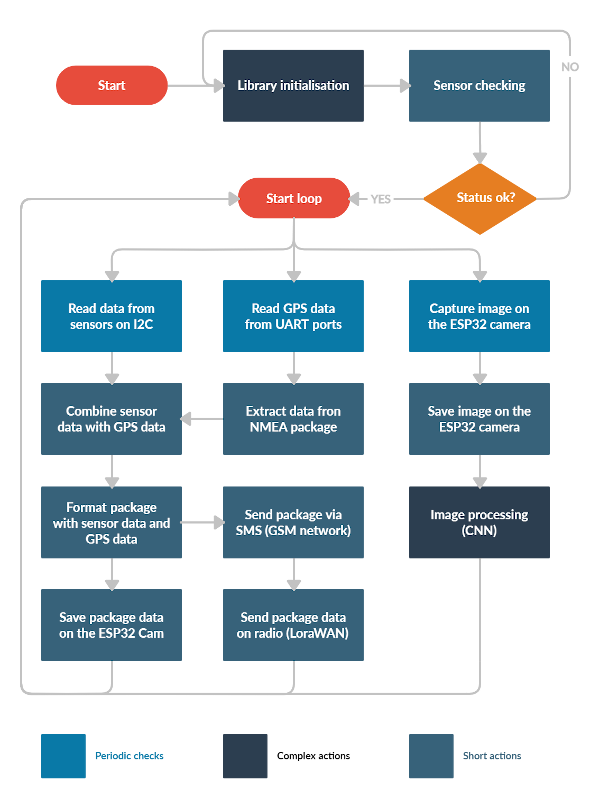
\includegraphics[width=12.7cm]{images/img_Code_Blocks.png}
    \caption{\small{Software diagram.}}
    \label{fig:codeblocks}
\end{figure}


The ESP32 microcontroller will be programmed using the C programming language and the official Espressif IoT Development Framework (ESP-IDF). To manage the SDK, the framework, and all the required tools, such as the compiler, we will be using PlatformIO for Visual Studio Code. This provides a user-friendly interface for managing the build process, and also allows us to integrate with other development tools such as Git for code versioning.

We will be using GIT extensively to keep track of changes to the codebase. Every time a new functionality is added to the code, Git takes a snapshot of the entire codebase. This allows us to easily roll back to a previous version if a new feature breaks the code. With Git, we can collaborate on the codebase and track changes made by different team members, ensuring a smooth and efficient development process.

\begin{wrapfigure}{r}{0.5\textwidth}
    \centering
    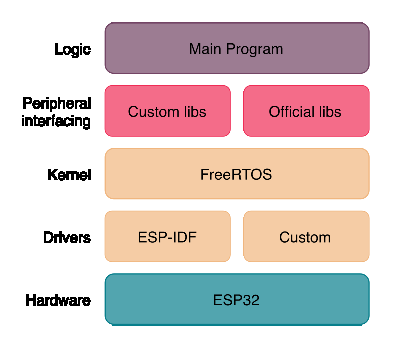
\includegraphics[width=7.5cm]{images/img_Cansat_RTOS.eps}
    \caption{\small{CanSat software state diagram.}}
    \label{fig:rtos}
\end{wrapfigure}



Additionally, we are planning to develop a custom software application that will run on the ground station. This application will receive the telemetry data from the CanSat and interpret it, visualizing the information on real-time graphs. The software will extract sensor data such as acceleration, GPS coordinates, pressure, and more from the raw data packets, allowing us to monitor the CanSat's performance and the environmental conditions it encounters. The software will also log the data to ensure that no valuable measurements are lost. This custom software will provide a vital tool for our team to monitor and analyze the CanSat's data during the mission.

\subsection{Recovery system}
Recovering the satellite is essential as extended mission data and video data are stored on the
CanSat. To ensure the safe and efficient recovery of the CanSat, a total of four systems were designed and implemented. 

Firstly, a parachute system was incorporated to slow down the descent rate and ensure a soft landing. Secondly, a radio beacon and buzzer were included to aid in locating the CanSat once it landed. Thirdly, a GSM messaging system was added to transmit the GPS coordinates to the recovery team. This allows for the rapid location and retrieval of the CanSat after landing. Overall, these four systems work in conjunction to ensure a successful and safe recovery mission.

\subsubsection{Parachute}
The parachute system was designed to slow down the descent rate of the CanSat to a safe and controlled speed, depending on weather conditions. To ensure the success of the recovery process, the design of the parachute system considers both the need for a longer flight time to conduct accurate atmospheric analysis during the descent phase in good weather conditions, as well as the need for a fast descent in case of bad weather conditions. It is worth noting that the calculations used to determine the descent rate also take into account the time factor, which is crucial for a successful recovery.

The hemispherical parachute with an additional spill hole of diameter $d=20\%$ of the canopy's diameter, $D$, on the top is our preferred primary recovery system due to its high drag coefficient per area, which allows for a lightweight parachute. This spill hole helps with air transition along the parachute, preventing CanSat oscillations during descent. Additionally, this parachute has been used in previous competitions with good results. 

Upon release from the rocket/airplane/helicopter, the parachute will immediately deploy to slow the CanSat's descent through the atmosphere. To stabilize the rotation of the CanSat during descent and obtain better camera images, the parachute will be connected to the can in six points using a lightweight rope weighing only 1 gram/meter.

It is recommended to connect canopy lines to the CanSat using a ball-bearing swivel. This will help prevent line entanglement during deployment and descent. Additionally, the length of the canopy lines should be 20\% longer than the radius of the canopy to prevent the lines from tangling during descent.

To account for different weather conditions, we have prepared three different parachutes. The first is designed for high-speed descent in bad weather conditions, allowing for a descent speed of 11-12 m/s. The second parachute is suitable for normal conditions, with a descent speed range of 7-10 m/s. The third parachute is intended for clear sky and no wind conditions, resulting in a descent speed of 5-6 m/s.

\begin{wrapfigure}{l}{0.26\textwidth}
    \centering
    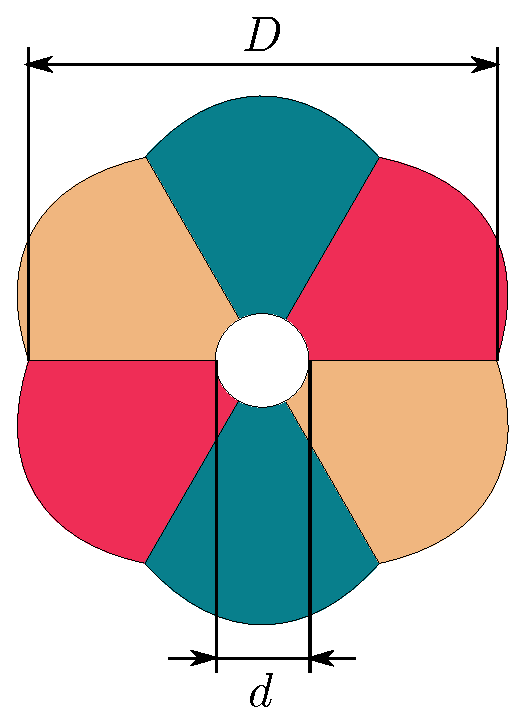
\includegraphics[width=4cm]{images/img_canopy2.eps}
    \caption{\small{Parachute design.}}
    \label{fig:software_fiagram}
\end{wrapfigure}

As we know, a falling object in a fluid (the atmosphere) is subject to two main forces:
\begin{itemize}[leftmargin=1cm,itemindent=0.5cm,noitemsep, topsep=4pt, label=$\bullet$]
    \item Weight $W = m \cdot g$ where $m = 0.3\text{ kg}$ and $g$ is the gravitational acceleration
    \item Friction $F_f = -k \cdot v^2$ where $k$ is the air friction coefficient ($\displaystyle k = \frac{\rho C_D A}{2}$) and $v$ is the velocity of the CanSat. Here, $\rho$ is the density of air, $C_D$ is the drag coefficient, $A$ is the parachute's area, and $v$ is the velocity in meters per second (m/s).
\end{itemize}

The resulting force on the CanSat is given by:
\begin{equation*}
F = W + F_f = mg - kv^2
\end{equation*}
Hence, we can obtain the expression for the terminal velocity, and consequently, the formula for the parachute's area, which leads to the equation for the diameter, D, of the canopy:
\begin{equation*}
v = \sqrt{\frac{2mg}{\rho C_D A}},\quad\quad A=\frac{2mg}{C_D \rho v^2}, \quad\quad D = \sqrt{\frac{8A}{n \sin\left(\frac{2\pi}{n}\right)}}
\end{equation*}


To calculate the dimensions required for the parachute, we considered the following constant parameters, including physical constants and canopy parameters.

\begin{table}[htbp]
\centering
\arrayrulecolor{DeepSkyBlue4}
\begin{tabular}{>{\centering\arraybackslash}lc}
\rowcolor{DeepSkyBlue4}
\hline
\multicolumn{1}{|c|}{\textbf{\color{white!50}{Parameter}}}  & \textbf{\color{white!50}{Value}} \\
\hline
$g$ - gravitational acceleration & \SI{9.81 }{\meter\per\square\second} \\
\rowcolor{LightCyan1!50}$\rho$ - air density & \SI{1.225}{\kilogram\per\cubic\metre} \\
$v$ - descent velocity & 6,9 and 12 \SI{}{\meter\per\second} \\
\rowcolor{LightCyan1!50}$m$ - CanSat mass & \SI{0.3}{\kilogram} \\
$C_D$ - Drag coefficient & 0.75 \\
\rowcolor{LightCyan1!50}$n$ - number of gores & 6 \\
\hline
\end{tabular}
\caption{Constant parameters and their values}
\end{table}

\subsubsection{Buzzer and GSM Messaging}
We have implemented two secondary recovery systems for the CanSat, to ensure its safe retrieval on the ground. The first system comprises two types of live telemetry, namely GSM and RF. This system transmits important data such as GPS coordinates, heading information from multiple sensors, and descent speed. The second recovery system is designed to aid in the precise localization of the CanSat using audio signals, which include a loud buzzer and a ribbon attached to the CanSat. This system is activated immediately after landing.

\subsection{Ground support equipment}
The ground segment software is a critical component that receives and processes data sent from the CanSat. This software is responsible for collecting, storing, and presenting the data in a user-friendly format. In addition, it provides advanced functionality for analyzing and visualizing the data, enabling the team to extract valuable insights and make informed decisions.

Our ground support equipment comprises receiver equipment and data visualization/logging components. The receiver equipment captures radio signals and telemetry data transmitted by the CanSat, and to ensure the best data quality, the receiver antennas will be mounted at a height of 2-3 meters above ground level. For ease of interpretation of the received data, we will be using multiple devices, including one or two omnidirectional antennas, a cell phone for SMS, and a laptop for RF telemetry with real-time graphs and data logging capabilities.

To ensure minimal packet loss, we have included an omnidirectional Moxon antenna and a 1/4 Wave Ground Plane Antenna in our ground station setup. These antennas will be linked to the ground stations and have the capability to maintain a strong signal even at a maximum distance of 1000 meters.

The CanSat LoRa and the ground station will operate on a frequency of 868.1 MHz, which is a free frequency band available for unlicensed use in many countries. This frequency band offers good propagation characteristics and is well-suited for long-range communication, making it a popular choice for IoT and other wireless applications.

To ensure that the software is able to capture all relevant data, it is designed to work seamlessly with the radio receiver. It processes the data in real-time, which means that the team can monitor the CanSat's progress and take action if necessary. Furthermore, the software is optimized for efficiency and reliability, ensuring that the data is stored safely and accurately.

The data received from the CanSat is stored in a file format that is easily readable and processable. To achieve this, we are using the CSV (Comma Separated Values) format, which allows for easy integration with various data analysis software tools. The CSV format also ensures that the data is organized and structured for efficient processing and analysis.

One of the key features of the software is its ability to present data in a user-friendly format. It provides clear, concise visualizations that allow the team to quickly identify trends and patterns in the data. This is crucial for making informed decisions and optimizing the CanSat's performance.

In addition to visualizing data, the software also provides advanced functionality for analyzing and processing data. This enables the team to extract valuable insights from the data, such as identifying areas for improvement or optimizing performance. The software also supports data logging, which ensures that all data is stored securely and can be accessed at a later time if necessary.

Overall, the ground segment software is an essential component that enables the team to maximize the performance of the CanSat. Its real-time data processing, clear visualizations, and advanced functionality make it a powerful tool for optimizing the CanSat's performance and achieving the mission's objectives.


\section{Project planning}
Effective project planning is essential for the successful design and construction of our proposed CanSat. From the outset, our team established a series of milestones that must be achieved during the competition phases. Accomplishing these milestones requires specific tasks, such as acquiring financial resources, identifying the most suitable materials, selecting high-performance sensors, and sourcing electronic components. Therefore, through discussions and careful planning, we have established a comprehensive plan to ensure the success of our CanSat project.

Our timeline takes into account every aspect of the project, including report writing, design, construction, launch, and testing. We have carefully allocated the necessary time and resources to each stage of the project to ensure that we meet our deadlines and achieve our goals. Regular progress checks will be conducted to ensure that we stay on track and make any necessary adjustments to our plan.

In addition to our internal timeline, we have also taken into consideration external factors, such as competition deadlines and launch availability, to ensure that we meet all necessary requirements and complete the project within the given timeframe.

By following our comprehensive timeline and adhering to our milestones, we are confident that we will successfully design, build, launch, and test our CanSat project.

\subsection{Time schedule of the CanSat preparation}\label{time_schedule}
To obtain a comprehensive understanding of our project's timeline, please refer to the Gantt Chart included in Appendix \ref{A1}. Alongside this chart, we have also compiled a list of extended milestones which outline achievable tasks and key performance indicators. 

These milestones have been designed to keep us on track and ensure that we successfully meet our project goals and deadlines.
\begin{itemize}[leftmargin=1cm, itemindent=0.25cm, noitemsep, topsep=0pt, label=$\bullet$]
    \item Team Formation and Project Planning:
    \begin{itemize}[label=\ding{111}, noitemsep, topsep=2pt]
        \item Establish team roles and responsibilities
        \item Recruit suitable team members for each role
    \end{itemize}
    \item Define Project Scope and Objectives:
    \begin{itemize}[label=\ding{111}, noitemsep, topsep=2pt]
        \item Purpose of the project: to successfully land and analyze the environment, light conditions, and terrain types to determine if it is a habitable environment
        \item Objectives to be achieved on launch day and post-launch analysis:
        \begin{multicols}{2}
        \setlength{\topsep}{2pt}
        \setlength{\partopsep}{0pt}
        \begin{itemize}[label=\ding{51}, noitemsep, topsep=0pt]
        \item Successful launch
        \item Live RF telemetry
        \item GSM Data
        \item Successful parachute deployment
        \item All systems nominal (good sensor and location data)
        \item Descent rate between 5-10m/s
        \item Landing confirmation
        \item Recovery of the CanSat
        \item Retrieval of images and telemetry data
        \item AI data analysis
        \item Generating reports
        \end{itemize}
        \end{multicols}
    \end{itemize}
    \item Develop a Detailed Project Plan and Timeline:
    \begin{itemize}[label=\ding{111}, noitemsep, topsep=2pt]
        \item Assign tasks related to social media promotion and sponsor search;
        \item Determine cooperation method (online/programs/meetings etc.)
    \end{itemize}
    \item Research and Design:
    \begin{itemize}[label=\ding{111}, noitemsep, topsep=2pt]
        \item Conduct research on required components and technologies for the CanSat;
        \item Design the CanSat's structure and select materials;
        \item Source the required sensors and electronics;
        \item Submit Preliminary Design Report;
        \item Develop a prototype and test sensors and electronics;
        \item Promote the project on social media platforms and begin searching for sponsors.
    \end{itemize}
    \item Integration and Testing:
    \begin{itemize}[label=\ding{111}, noitemsep, topsep=2pt]
        \item Integrate sensors and electronics into the CanSat's structure;
        \item Conduct system-level testing and calibration;
        \item Ensure that the CanSat meets weight and size requirements;
        \item Continue promoting the project on social media platforms and searching for sponsors.
    \end{itemize}
    \item Launch Preparation:
    \begin{itemize}[label=\ding{111}, noitemsep, topsep=2pt]
        \item Conduct pre-launch testing;
        \item Pre-launch checklist.
    \end{itemize}
    \item Primary Mission:
    \begin{itemize}[label=\ding{111}, noitemsep, topsep=2pt]
        \item Verify that the CanSat met the primary mission requirements;
        \item Share updates and photos of the launch on social media platforms.
    \end{itemize}
    \item Secondary Mission:
    \begin{itemize}[label=\ding{111}, noitemsep, topsep=2pt]
        \item Collect air quality, light intensity, and surface terrain state data;
        \item Define data interpretation criteria and relevant data from sensors;
        \item Train an AI to analyze image data transmitted from the CanSat;
        \item Conduct data analysis and report on the results;
        \item Share updates and photos of the data analysis on social media platforms.
    \end{itemize}
    \item Submit Design Reviews
    \begin{itemize}[label=\ding{111}, noitemsep, topsep=2pt]
        \item Preliminary Design Review;
        \item Critical Design Review.
    \end{itemize}
    \item Final Report and Presentation:
    \begin{itemize}[label=\ding{111}, noitemsep, topsep=2pt]
    \item Prepare a final report documenting the project's objectives, methods, and results;
    \item Develop a presentation to showcase the CanSat and its capabilities;
    \item Present the final report and presentation to the project stakeholders;
    \item Share the presentation on social media platforms to showcase the project's achievements and thank sponsors for their support.
    \end{itemize}
\end{itemize}

By achieving these milestones, we will ensure the success of our CanSat project and meet our project goals and deadlines.

\section{Risks analysis and mitigation}
The risk analysis section is an essential part of any project plan. In this section, we identify potential risks that may impact the success of the CanSat mission and develop strategies to mitigate those risks. This itemized list provides a summary of the significant risks we have identified and the steps we have taken to address them.

\begin{itemize}[leftmargin=1cm, itemindent=0.25cm, noitemsep, topsep=0pt, label=$\bullet$]
\item \textbf{Launch vehicle failure}: Can result in the loss of the CanSat and its mission. Ensure that the CanSat is designed to withstand launch loads and the launch vehicle is reliable. No contingency plans for this scenario, organizers should provide a different means for launch if needed.
\item \textbf{Communication failure}: Critical for mission success. Factors such as interference, distance, and line of sight can impact the quality and reliability of the communication link. Mitigate risks through system checks, tests, and system deployment procedures with a checklist. Onboard self-diagnostics and visual confirmation through an addressable LED. 2 GPS systems and 3 telemetry systems on different radio frequencies to transmit data separately.
\item \textbf{Power limitations}: CanSat is limited in terms of the amount of power that it can generate and store. Ensure that the CanSat is designed to be power-efficient and has sufficient power to complete its mission. Detailed power budget that takes into account real-life battery capacity and energy needs of all modules.
\item \textbf{Environmental factors}: CanSat will be subjected to a range of environmental factors such as temperature, humidity, and vibration during launch and operation. Ensure that the CanSat is designed to withstand these conditions and that the mission objectives are achievable under these conditions. Endurance tests in different environments, simulation of high G forces, and landing tests.
\item \textbf{Technical issues}: Can arise during the design, integration, testing, and operation of the CanSat. Prototype the CanSat development board to pre-assemble a fully functioning CanSat and catch any mistakes that were introduced in the design before building the final CanSat. Identify potential technical issues early and have contingency plans in place to address them. 
\item \textbf{Budget constraints}: CanSat projects are often subject to budget constraints. Ensure that the project is feasible within the available budget and prioritize mission objectives accordingly. Detailed budget with part of it covered by a sponsor, and constantly on the lookout for new sponsors. Committed to supporting the cost from personal finances if no new sponsors are found.
\end{itemize}

\subsection{Resource estimation}
To ensure that the project is completed successfully within the given budget and timeframe, it is crucial to perform a thorough estimation of the required resources. This includes identifying the necessary materials, equipment, and team members needed to complete the project, as well as the associated costs and time requirements. 

By performing a detailed resource estimation, the project team can effectively plan and allocate resources to ensure that the project is completed on time, within budget, and to the desired quality standards. 

Below is a breakdown of the resources required for the CanSat project:
\begin{itemize}[leftmargin=1cm, itemindent=0.25cm, noitemsep, topsep=0pt, label=$\bullet$]
\item Materials and components:
\begin{itemize}[label=\ding{111}, noitemsep, topsep=1pt]
\item Identify and list out all the required materials and components, including a microcontroller, sensors, batteries, antennas, radio modules, lightweight printable plastics, and other miscellaneous parts
\item Cost of materials can vary depending on the quality and quantity of components required
\end{itemize}
\item Tools and equipment:
\begin{itemize}[label=\ding{111}, noitemsep, topsep=1pt]
\item Various tools and equipment required, such as multimeters, 3d printers, oscilloscope, soldering station, and other miscellaneous parts
\end{itemize}
\item Software:
\begin{itemize}[label=\ding{111}, noitemsep, topsep=1pt]
\item Programming microcontrollers, designing 3D concepts, and analyzing data collected by the sensors
\item Using open-source software can significantly reduce the costs associated with software for the project. This option is preferable to purchasing software, which can be costly.
\end{itemize}
\item Manpower and build time:
\begin{itemize}[label=\ding{111}, noitemsep, topsep=1pt]
\item An essential component of the project
\item Online tools and weekly meetings are used to ensure accuracy
\item Estimated effort of 630 hours for the entire project.
\end{itemize}
\item Testing and validation:
\begin{itemize}[label=\ding{111}, noitemsep, topsep=1pt]
\item Essential step to ensure the project performs as expected
\item May include the use of specialized equipment such as a drone or rocket
\end{itemize}
\item Shipping, transport, and logistics:
\begin{itemize}[label=\ding{111}, noitemsep, topsep=1pt]
\item Shipping and logistics costs may need to be factored into the project’s budget
\item May include shipping materials and components and travel costs for team members to attend the competition
\end{itemize}
\item Miscellaneous costs:
\begin{itemize}[label=\ding{111}, noitemsep, topsep=1pt]
\item Other costs that may need to be considered when estimating resources for the CanSat project
\end{itemize}
\end{itemize}

In conclusion, it is evident that a successful project outcome is heavily reliant on a proper estimation of resources required to complete the project. Neglecting the factors such as materials, components, tools, equipment, software, testing and validation, shipping and logistics, and other unforeseen costs can lead to budget overruns, delays, and ultimately failure to achieve project objectives.

\subsubsection{Budget}

We conducted thorough research to ensure that our budget aligns with the ideal specifications for our CanSat. This involved finding the most efficient and lightweight components without compromising performance, as well as maximizing battery life. By carefully considering each part, we aimed to optimize our budget and ensure that we could achieve our project objectives.

However, building the CanSat is just a part of the project. Therefore, our budget covers the entire project from start to finish, which can be divided into four main parts: 
\begin{itemize}[leftmargin=1cm, itemindent=0.25cm, noitemsep, topsep=0pt, label=$\bullet$]
    \item \textbf{Hardware parts}: all the necessary mechanical and electronic/electrical parts required to build both our custom development board and final CanSat. The cost estimation includes the purchase of a microcontroller, sensors, batteries, antennas, radio modules, lightweight printable plastics, and other miscellaneous parts.
    \item \textbf{Publicity and Branding}: covers the creation of custom t-shirts to promote our team and the event. In addition to custom t-shirts, we will also invest in creating promotional materials such as flyers, posters, and banners that showcase our team and the CanSat mission. These materials will be distributed both digitally and in person to help increase awareness of our project and the competition. Additionally, we will allocate a portion of our budget towards branding efforts such as website design and social media management to maintain a consistent and professional image for our team. Investing in Publicity and Branding will help us build a strong reputation within the community and attract potential sponsors and supporters to our cause.
    \item \textbf{Travel Expenses}: includes the transportation costs, with tickets for the team to travel to the Competition Venue. This includes the cost of transportation by train, as well as any necessary local travel expenses.
    \item \textbf{Emergency Funds}: a contingency budget to cover any unforeseen costs that may arise during the project.
\end{itemize}

Below is a table that outlines all the anticipated expenses associated with the CanSat mission. This includes the costs of the components used to construct the CanSat, as well as any supplementary materials, equipment, and personnel necessary to complete the mission.

The components required for the project were purchased from various suppliers such as Amazon, Mouser, TME, Adafruit, and JLCPCB. It is worth noting that the team did not receive Cansat kits, and as a result, the team members did all the design and construction of the CanSat.

\begin{table}[htbp]
\centering
\arrayrulecolor{DeepSkyBlue4}
\begin{tabular}{>{\centering\arraybackslash}p{4.5cm}>{\centering\arraybackslash}lc}
\rowcolor{DeepSkyBlue4}
\hline
\multicolumn{1}{c}{\textbf{\color{white!50}{Category}}}& \multicolumn{1}{c}{\textbf{\color{white!50}{Cost Item}}} & \textbf{\color{white!50}{Cost \texteuro}} \\
\hline
\multicolumn{1}{l}{Hardware Parts (383\texteuro)}& ESP32-S3-WROOM ($\mu$C) & 6 \\
& \cellcolor{LightCyan1!50}ESP32Cam board ($\mu$C)& \cellcolor{LightCyan1!50}9 \\
& Arduino Nano 33 BLE Sense ($\mu$C)& 29 \\
& \cellcolor{LightCyan1!50}AltIMU-10 v5 - IMU Sensor & \cellcolor{LightCyan1!50}25 \\
& MPU 6050 - IMU Sensor & 5 \\
& \cellcolor{LightCyan1!50}BME688 - Barometric Pressure & \cellcolor{LightCyan1!50}10 \\
& BME280- Barometric Pressure & 10 \\
& \cellcolor{LightCyan1!50}MCP9808 - Temperature Sensor & \cellcolor{LightCyan1!50}5 \\
& VEML6075 - UVA UVB UV Sensor & 5 \\
& \cellcolor{LightCyan1!50}VEML7700 - UV Sensor & \cellcolor{LightCyan1!50}4 \\
& GUVA-S-12-D - UV Sensor & 6 \\
& \cellcolor{LightCyan1!50}SPS30 - Environmental Sensor & \cellcolor{LightCyan1!50}45 \\
& SCD40 - Environmetal Sensor & 30 \\
& \cellcolor{LightCyan1!50}NEO-M9N - GPS & \cellcolor{LightCyan1!50}25 \\
& Quectel L76 - GPS & 10 \\
& \cellcolor{LightCyan1!50}PCB components (RLC, diodes) & \cellcolor{LightCyan1!50}10 \\
& Power Switching regulators & 4 \\
& \cellcolor{LightCyan1!50}micro SD & \cellcolor{LightCyan1!50}6 \\
& 64Mb Flash memory & 8 \\
& \cellcolor{LightCyan1!50}SIM800L - GSM Module & \cellcolor{LightCyan1!50}12 \\
& Buzzer & 1 \\
& \cellcolor{LightCyan1!50}Antennas & \cellcolor{LightCyan1!50}30 \\
& SMA Connectors & 3 \\
& \cellcolor{LightCyan1!50}Radio modules & \cellcolor{LightCyan1!50}30 \\
& Parachute material & 24 \\
& \cellcolor{LightCyan1!50}Parachute cords & \cellcolor{LightCyan1!50}6 \\
& Battery & 25 \\
\multicolumn{1}{l}{Publicity \& Branding (100 \texteuro)}& \cellcolor{LightCyan1!50}T-Shirts & \cellcolor{LightCyan1!50}65 \\
& 3D printer filament & 15 \\
& \cellcolor{LightCyan1!50}Flyers \& stickers & \cellcolor{LightCyan1!50}20 \\
\multicolumn{1}{l}{Travel Expenses (315 \texteuro)} & Train tickets & 205 \\
& \cellcolor{LightCyan1!50} Meals & \cellcolor{LightCyan1!50}110 \\
\multicolumn{1}{l}{Emergency Funds}& Miscellaneous & 100 \\
\hline
& \textbf{Total} & \textbf{898} \\
\hline
\end{tabular}
\caption{Foreseen costs for the CanSat mission.}
\label{tab:costs}
\end{table}




\subsubsection{External support}
The successful execution of the CanSat mission relies on the assistance and resources given by different organizations, departments, and companies. We are fortunate to have received sponsorship or in-kind support from the following entities:
\begin{itemize}[leftmargin=1cm, itemindent=0.25cm, noitemsep, topsep=0pt, label=$\bullet$]
    \item \textbf{CoderDojo Oradea} has provided substantial financial aid, technical support, and feedback on both hardware and software. This makes them our biggest sponsor so far, allowing us to acquire all of the most expensive components of our CanSat and facilities where we can carry out our activities;
    \item \textbf{Funda\c{t}ia Comunitar\u{a} Oradea} has generously provided facilities where we can conduct our activities;
    \item \textbf{EduTrust} has provided both financial support and working facilities for our team;
    \item \textbf{Elektrobit} has provided financial support, access to facilities, equipment, and expertise in Embedded systems;
    \item \textbf{Depozitul de Tricouri} has agreed to provide customized T-shirts for each team member, which will help us promote our team and the event.
\end{itemize}


\subsection{Test plan}

The success of a CanSat mission depends on the thorough testing of the system before the launch. This test plan outlines the various tests that will be conducted to ensure that the CanSat meets the mission objectives and functions properly under different conditions. The tests are categorized into mechanical, software, payload, communication, power, environmental, integration, ground station, battery charging, launch, and post-mission tests. The goal of these tests is to ensure that the CanSat is capable of collecting and transmitting data accurately, withstand the harsh environmental conditions, and survive the launch and landing phases. The following is a roadmap for testing the CanSat, with general ideas for each test.

\begin{itemize}[leftmargin=1cm, itemindent=0.25cm, noitemsep, topsep=0pt, label=\ding{51}]
\item Mission Objective Test
\begin{itemize}[label=\ding{111}, noitemsep, topsep=2pt]
\item Verify if the CanSat meets the competition mission requirements
\item Check that the sensors are functioning properly
\end{itemize}

\item Mechanical Test
\begin{itemize}[label=\ding{111}, noitemsep, topsep=2pt]
\item Make sure that the structure and enclosure are sturdy and can withstand launch and landing
\item Verify the parachute deployment and fixing are functional and reliable
\item Optimize and check if the shock-absorbing system can protect the system from damage during the landing
\end{itemize}

\item Software Test
\begin{itemize}[label=\ding{111}, noitemsep, topsep=2pt]
\item Verify that the software is correctly installed and functional
\item Ensure that the software is properly processing data from the sensors and instruments
\end{itemize}

\item Payload Test
\begin{itemize}[label=\ding{111}, noitemsep, topsep=2pt]
\item Ensure that the sensor data is being transmitted correctly
\item Check the accuracy of the sensor data being transmitted
\item Verify if the parachute system is working properly
\end{itemize}

\item Communication Test
\begin{itemize}[label=\ding{111}, noitemsep, topsep=2pt]
\item Ensure that the CanSat can communicate with the ground station
\item Verify that telemetry data can be received and decoded correctly
\item Test the range of the communication link
\item Check the reliability of the communication link
\end{itemize}

\item Power Test
\begin{itemize}[label=\ding{111}, noitemsep, topsep=2pt]
\item Verify that the power system meets the power budget and has sufficient power to operate the CanSat
\item Test the duration of the battery life
\item Ensure that power consumption is minimized wherever possible
\end{itemize}

\item Environmental Test
\begin{itemize}[label=\ding{111}, noitemsep, topsep=2pt]
\item Verify if the CanSat can withstand the range of environmental conditions that it will be exposed to during the mission
\item Test the CanSat in extreme temperature and humidity conditions
\item Test the CanSat's ability to withstand vibration and shock
\end{itemize}

\item Integration Test
\begin{itemize}[label=\ding{111}, noitemsep, topsep=2pt]
\item Verify if all the components of the CanSat are properly integrated and functioning correctly
\item Test the overall functionality of the CanSat
\end{itemize}

\item Ground Station Test
\begin{itemize}[label=\ding{111}, noitemsep, topsep=2pt]
\item Verify that the antennas are properly installed and functional
\item Ensure that the ground station software can receive data from the CanSat
\item Verify that the ground station software can display data from the CanSat
\end{itemize}

\item Battery Charging Test
\begin{itemize}[label=\ding{111}, noitemsep, topsep=2pt]
\item Test the battery charging system and verify that it can fully charge the batteries within a reasonable amount of time
\item Verify that the charging system is safe and reliable
\end{itemize}

\item Launch Test
\begin{itemize}[label=\ding{111}, noitemsep, topsep=2pt]
\item Verify that the CanSat can survive the launch environment
\item Test the recovery system, ensuring that the CanSat lands safely
\end{itemize}

\item Post-Mission Test
\begin{itemize}[label=\ding{111}, noitemsep, topsep=2pt]
\item Verify if the CanSat has returned all the required data
\item Check the data for accuracy and completeness
\item Analyze the data and compare it to the mission objectives
\end{itemize}

\end{itemize}

The general test list provides a roadmap for ensuring that the CanSat meets the competition requirements and can perform its intended mission. However, to ensure the CanSat's success, conducting more specific tests on its electronics and structure is crucial. These tests will verify that the sensors and instruments are functioning correctly and that the CanSat's structure can withstand the rigors of launch, landing, and environmental conditions. 

\begin{itemize}[labelwidth=0cm, leftmargin=0cm, itemindent=0.7cm, noitemsep, topsep=0pt, label={}]
\item \textbf{Pressure sensor test}:
\begin{itemize}[labelwidth=2cm, leftmargin=1.9cm, label=\ding{109}, noitemsep, topsep=2pt]
\item[\faTasks] \textbf{Task}: Expose the used sensor to a pressure change and compare the results with a reference device.
\item[\faFlask] \textbf{Method}: Place the target and reference sensors in a sealed container with a known volume of air and measure the pressure change with a manometer or a barometer. The pressure can be changed by altering the volume of the container or by using a hand pump.
\item[{\faHourglass[3]}] \textbf{Estimated testing time duration}: 1-2 hours
\item[{\faCheckSquare}] \textbf{Acceptance criteria}: The test will be considered positive when both sensors show the same pressure without measuring errors.
\end{itemize}
\item \textbf{Temperature sensor test}:
\begin{itemize}[labelwidth=2cm, leftmargin=1.9cm, label=\ding{109}, noitemsep, topsep=2pt]
\item[\faTasks] \textbf{Task}:  Check whether the target device and the reference device show the same temperature within 24 hours 
\item[\faFlask] \textbf{Method}: Place both the target device and the reference device in the same location and monitor their temperature readings at regular intervals for 24 hours
\item[{\faHourglass[3]}] \textbf{Estimated testing time duration}:  24 hours
\item[{\faCheckSquare}] \textbf{Acceptance criteria}: The test will be considered positive when both sensors show the same temperature without significant deviation.
\end{itemize}
\item \textbf{Humidity sensor test}:
\begin{itemize}[labelwidth=2cm, leftmargin=1.9cm, label=\ding{109}, noitemsep, topsep=2pt]
\item[\faTasks] \textbf{Task}:  Place the target sensor and the reference device in a humidity chamber where the humidity will be increased or decreased to a specific level, and the readings will be compared.
\item[\faFlask] \textbf{Method}: The target sensor and the reference device will be placed in a humidity chamber where the humidity level will be gradually increased or decreased to a specific level. The readings from both sensors will be recorded and compared.
\item[{\faHourglass[3]}] \textbf{Estimated testing time duration}:  6 hours
\item[{\faCheckSquare}] \textbf{Acceptance criteria}: The test will be considered positive when both sensors show the same humidity level without significant deviation.
\end{itemize}
\item \textbf{UV sensor test}:
\begin{itemize}[labelwidth=2cm, leftmargin=1.9cm, label=\ding{109}, noitemsep, topsep=2pt]
\item[\faTasks] \textbf{Task}:  Expose the target sensor and the reference device to UV radiation from a UV light source and compare the readings.
\item[\faFlask] \textbf{Method}: The target sensor and the reference device will be exposed to UV radiation from a UV light source for a specific duration, and the readings will be recorded and compared.
\item[{\faHourglass[3]}] \textbf{Estimated testing time duration}:  1 hour
\item[{\faCheckSquare}] \textbf{Acceptance criteria}: The test will be considered positive when both sensors show the same UV index without significant deviation.
\end{itemize}
\item \textbf{GPS test}:
\begin{itemize}[labelwidth=2cm, leftmargin=1.9cm, label=\ding{109}, noitemsep, topsep=2pt]
\item[\faTasks] \textbf{Task}:  Test the accuracy of the GPS module by comparing the location obtained by the CanSat with the actual location.
\item[\faFlask] \textbf{Method}: The location data collected by the GPS module during this time will be recorded and compared to the actual location using a separate reference system. The reference system may be a ground-based GPS receiver or a separate device with accurate location data.
\item[{\faHourglass[3]}] \textbf{Estimated testing time duration}:  1 hour
\item[{\faCheckSquare}] \textbf{Acceptance criteria}: The test will be considered positive if the error margin is within an acceptable range.
\end{itemize}
\end{itemize}

Endurance tests are an essential part of the CanSat testing process as they are designed to assess the satellite's ability to withstand the harsh environmental conditions it may encounter during a typical mission. These tests are conducted to ensure that the CanSat components can withstand the forces of a fall, vibration, shock, and prolonged exposure to G-forces during rocket transport. Additionally, the endurance tests provide valuable information about the limits of the CanSat and its performance under different conditions. 

\begin{itemize}[labelwidth=0cm, leftmargin=0cm, itemindent=0.7cm, noitemsep, topsep=0pt, label={}]
\item \textbf{Drop resistance test}:
\begin{itemize}[labelwidth=2cm, leftmargin=1.9cm, label=\ding{109}, noitemsep, topsep=2pt]
\item[\faTasks] \textbf{Task}: Conduct a crash test to ensure the CanSat components can withstand the impact of a fall.
\item[\faFlask] \textbf{Method}: Prototypes will be dropped from a tower or drone to achieve the required descent speed. A fall test without a parachute will also be performed. Optionally, a 3-axis accelerometer will be added to record any G-force during the test.
\item[{\faHourglass[3]}] \textbf{Estimated testing time duration}: Estimated to be a few hours.
\item[{\faCheckSquare}] \textbf{Acceptance criteria}: All components should remain intact, and the electronics should continue to work continuously.
\end{itemize}
\item \textbf{Long-term G-force tests}:
\begin{itemize}[labelwidth=2cm, leftmargin=1.9cm, label=\ding{109}, noitemsep, topsep=2pt]
\item[\faTasks] \textbf{Task}: Simulate the G-forces that may occur during rocket transport to test the CanSat components' endurance.
\item[\faFlask] \textbf{Method}: The CanSat model will be placed on a carousel or string and rapidly rotated to generate the required overload due to the centrifugal force.
\item[{\faHourglass[3]}] \textbf{Estimated testing time duration}: The test will last for several hours.
\item[{\faCheckSquare}] \textbf{Acceptance criteria}: All components should remain intact, and the electronics should continue to work continuously throughout the test period.
\end{itemize}
\end{itemize}

By conducting both general and specific tests, the team can be confident that the CanSat is fully functional and prepared for a successful mission.


\subsection{Time management}
To ensure the project stays on track and meets the desired timeline, we have decided to utilize the web-based Gantt tool, \href{https://app.teamgantt.com/}{\color{DeepSkyBlue4}{TeamGantt.com}}. The project has been divided into several phases, with each phase having a specific duration and tasks to be accomplished.

The ideation phase has already been completed, and we are currently in the design and prototyping stages of the CanSat, with the remaining phases including various testing campaigns and construction runs. The exact details of the testing phase are yet to be defined and will be determined as the project progresses. The final phase will culminate in the competition. By using this tool, we can monitor progress, adjust timelines, and stay on schedule to achieve the desired outcomes

We estimate a total of 630 man-hours needed for the entire project, and we have already invested 330 hours towards it. The Gantt chart automatically updates as we progress through the project, allowing us to monitor our progress and adjust our plans as necessary to ensure the timely completion of the project.

We have started testing Jira in parallel with using TeamGantt.com to implement an Agile framework for future competitions. Jira is a project management software that provides a flexible and powerful platform for managing projects using an Agile framework. 

By implementing Jira, we can create a central location for tracking tasks, issues, and progress throughout the project lifecycle. This will allow us to easily collaborate and communicate with team members and stakeholders, as well as prioritize tasks and adjust schedules based on changing requirements or circumstances. In addition, Jira offers a range of reporting and analytics features, providing valuable insights into team performance, task completion rates, and potential bottlenecks. With Jira, we can also track time and effort spent on each task, which will help us better estimate future efforts and improve our planning and scheduling for future competitions. By using both Jira and TeamGantt.com, we can optimize our project management process and ensure efficient, effective completion of the CanSat project.

To ensure that we complete all necessary tasks on time, the following is a summary of our timeline. For a more detailed timeline, please refer to the Gantt chart provided in the Appendix.

\begin{itemize}[leftmargin=1cm, itemindent=0.25cm, noitemsep, topsep=0pt, label=$\bullet$]
\item Team formation: 01.02.2023 - 20.02.2023
\begin{multicols}{2}[\vspace{-0.75\baselineskip}]
\begin{itemize}[label=\ding{59}, noitemsep, topsep=2pt]
\item Think of feasible mission objectives and requirements
\item CanSat Application Work \& Registration
\end{itemize}
\end{multicols}
\vspace*{-0.75\baselineskip}
\item Ideation: 01.02.2023 - 10.05.2023
\begin{multicols}{2}[\vspace{-0.75\baselineskip}]
\begin{itemize}[label=\ding{59}, noitemsep, topsep=2pt]
\item Documentation writing (PDR, CDR, FDR)
\item Mission refinements
\end{itemize}
\end{multicols}
\vspace*{-0.75\baselineskip}
\item Design the CanSat: 21.02.2023 - 10.05.2023
\begin{multicols}{2}[\vspace{-0.75\baselineskip}]
\begin{itemize}[label=\ding{59}, noitemsep, topsep=2pt]
\item Mechanical structure 
\item Electrical system
\item Software
\item Recovery system
\item Ground support
\end{itemize}
\end{multicols}
\vspace*{-0.75\baselineskip}
\item Prototyping: 13.03.2023 - 17.04.2023
\item Testing (prototype): 10.04.2023 - 30.04.2023
\item Build the CanSat: 10.04.2023 - 30.04.2023
\item Launch Campaign: 10.05.2023 - 15.05.2003
\end{itemize}

Our program takes into account the potential issues that may arise at each phase and the time required to address them. However, unforeseen events may occur during the project, and as such, we have developed measures for prevention and risk mitigation, which are detailed below.

\begin{table}[htbp]
\centering
\arrayrulecolor{DeepSkyBlue4}
\begin{tabular}{>{\raggedright\arraybackslash}p{8cm}>{\raggedright\arraybackslash}p{7cm}}
\rowcolor{DeepSkyBlue4}
\hline
\multicolumn{1}{c}{\textbf{\color{white!50}{Major risks}}} & \multicolumn{1}{c}{\textbf{\color{white!50}{Mitigation}}} \\
\hline
Delays in obtaining mandatory materials and electronic components due to the global semiconductor chip shortage, resulting in unavailability and delivery delays & Place orders for materials and electronic components well in advance, find alternative components and adjust the project timeline accordingly \\
\rowcolor{LightCyan1!50}Overtime required for the electrical design part due to thorough testing and prototyping of the onboard circuits before integration into the final design & Create a good electrical schematic and perform exhaustive checks before beginning the physical build to catch any errors \\
Unforeseen technical difficulties that may require additional troubleshooting time and access to technical guidance from partners & Grant some extra time for troubleshooting and have access to technical guidance from our partners \\
\rowcolor{LightCyan1!50}Adverse weather conditions during testing & Analyze the weather status in advance and plan at least one backup day for testing \\
CanSat damage during testing due to inappropriate launch sites and lack of safety measures & Carefully choose the launch site when testing the CanSat and ensure that all safety measures are met \\
\rowcolor{LightCyan1!50}Recovery failure due to poor GPS transmission and weak buzzer sound & Before launching, ensure that the GPS transmission is strong and the buzzer sound is loud \\
Team member availability: Unexpected absences or departures of team members could delay the project and lead to workload imbalances & Clear communication and expectations among team members, cross-training team members on critical tasks, and having backup plans for key roles \\
\hline
\end{tabular}
\caption{Unforeseen events and risk mitigation.}
\label{tab:risks}
\end{table}

\section{Data Analysis and Outreach}
The data collected during the CanSat mission holds a wealth of information that can provide valuable insights into various aspects of the mission. Data analysis is, therefore, a crucial step in making sense of the collected data, drawing meaningful insights, and making informed decisions. In addition to analyzing the data for internal use, outreach is another important aspect of the data analysis process. Through outreach, the findings of the analysis can be shared with a wider audience, including stakeholders, the scientific community, and the public. In this section, we will discuss the data analysis and outreach efforts of the CanSat mission, highlighting the various tools and strategies used to analyze and disseminate the collected data.

\subsection{Data Analysis Plan}

The CanSat data plan is a comprehensive approach to collecting, processing and analyzing the data generated by the CanSat mission. The plan leverages various Python libraries to ensure that the data is acquired, processed, and visualized effectively. The six components of the data plan are Data acquisition, Data processing, Data visualization, Visual data processing, Pre-trainer software, and Statistical analysis.


\begin{itemize}[leftmargin=1cm,itemindent=0.5cm, noitemsep, topsep=0pt]
    \item \textbf{Data acquisition}: The data acquisition component of the plan utilizes a Python library to collect and store data from the CanSat sensors in real time. The library is designed to be compatible with the sensors used on the CanSat and is used to record data during the flight.
    \item \textbf{Data processing}: The data processing component of the plan involves a Python library that processes and cleans the raw data collected by the data acquisition software. The library is used to filter out any noise or errors in the data and organize it into a format suitable for analysis. To achieve the mission objectives, a range of statistical techniques and models, such as Stratonovich–Kalman–Bucy\endnote{\href{https://en.wikipedia.org/wiki/Kalman_filter}{https://en.wikipedia.org/wiki/Kalman\_filter}} filtering algorithms, will be employed to filter out noise and errors in the data. This will ensure that the data is accurate and reliable for further analysis.
    \item \textbf{Data visualization}: The data visualization component of the plan employs Python libraries such as Matplotlib and Seaborn to create visual representations of the data, such as easy-to-understand graphs and charts. These visualizations can help to quickly understand the data and identify patterns or trends.
    \item \textbf{Visual data processing}: This component of the plan is intended to analyze the images stored on the board of the CanSat using a pre-trained AI model. The model is developed using Python libraries such as TensorFlow and Keras. This component can aid in identifying the presence of geological features such as valleys, mountains, forests, and volcanoes, as well as potential signs of water or ice on the surface of a planet.
    \item \textbf{Pre-trainer software}: The pre-trainer software is an essential tool for developing accurate and effective AI models for visual data processing. The pre-trainer utilizes Python libraries such as Scikit-learn and PyTorch to collect photos, classify them into desired categories, and use them for training the AI model.
    \item \textbf{Statistical analysis}: The statistical analysis component of the plan uses Python libraries such as Pandas and Scipy to perform statistical analyses on the data. The library is used to identify any significant relationships or patterns in the data, such as the relationship between pressure and altitude. Statistical analysis is an essential tool for identifying trends and patterns in the data and drawing meaningful insights.
\end{itemize}

In addition to the software and tools used, the data analysis plan also outlines potential challenges and limitations that may arise during the analysis process. One such challenge is the need to account for external factors, such as atmospheric conditions, that may affect the accuracy of the data.

Another critical aspect of the data analysis plan is the documentation of the process to ensure transparency and reproducibility. The plan includes detailed descriptions of each step of the analysis process, including the software and tools used, any models or statistical techniques applied, and any assumptions or limitations of the analysis.

The use of statistical techniques and models, as well as powerful Python libraries for data manipulation and visualization, will enable the mission team to draw meaningful insights from the data and make informed decisions.

\subsection{Outreach Program}

Our outreach program has two primary objectives. The first is to promote the interrelated STEM disciplines, Science, Technology, Engineering, and Mathematics, and highlight their distinct but interconnected nature. These four fields are essential in shaping the future of technological advancements and scientific discoveries, and we aim to inspire the next generation to pursue careers in STEM-related fields.

The second objective of our outreach program is to popularize the space sector and space exploration. We aim to educate the public about the importance of space technologies and how they impact our daily lives. Furthermore, we want to showcase the role of CanSats in space exploration and highlight the various stages involved in their development, from design to launch. Through our outreach efforts, we hope to inspire the public to take an interest in space exploration and encourage the pursuit of careers in the space industry.

The team has developed a comprehensive plan for public engagement and education about the CanSat project. This outreach plan involves various activities to disseminate information about the project, including:
\begin{multicols}{2}[\vspace{-0.5\baselineskip}]
        \begin{itemize}[leftmargin=1cm,itemindent=0.5cm,noitemsep, topsep=0pt, label=$\bullet$]
%\begin{itemize}[, noitemsep, topsep=0pt]
\item presentations
\item workshops
\item demonstrations
\item social media
\item websites
\item community engagement
\item participation in science fairs or events.
\end{itemize}
\end{multicols}
\vspace*{-0.5\baselineskip}

In addition to outlining the different types of outreach activities that the team will undertake, it is essential to consider each activity's expected audience, message, medium, and outcome.

Presentations will be given to schools, community groups, and other organizations to educate people about the CanSat project and the technology used. Workshops will be organized to teach interested individuals about designing and building CanSats. Demonstrations will be provided to showcase the CanSat's capabilities in person or through videos or other media. The message will focus on the importance of STEM fields, the relevance of CanSat technology, and the process of designing and building a CanSat. The medium will include PowerPoint presentations and interactive demonstrations using physical models or simulators. The outcome of these activities will be to increase awareness and interest in the CanSat project and inspire the audience to pursue STEM-related fields.

Social media platforms such as Twitter, Instagram, and Facebook will be used to document the team's progress and share updates about the project with the public. A website will be developed to provide detailed information about the project, including updates on the progress, photos, videos, and data from the mission. The message will focus on providing regular updates about the CanSat project, including its progress, challenges, and successes. The medium will include text, photos, and videos posted on social media platforms. The outcome of these activities will be to increase engagement and interest in the CanSat project and to create a sense of community around it.

The team will also engage with the local community by visiting schools or community centers to talk about the project and its goals. In addition, they will participate in science fairs or events to showcase their CanSat design and educate people about the project. The message will focus on the importance of STEM fields and the potential of CanSat technology to inspire innovation and problem-solving. The medium will include interactive discussions, Q\&A sessions, and hands-on demonstrations of CanSat models or simulators. The outcome of these activities will be to foster a sense of community engagement and to increase interest and awareness of the CanSat project and STEM fields.

For science fairs or events, the target audience will be students, teachers, and members of the public interested in STEM education and space technology. The message will focus on showcasing the CanSat project and its potential to inspire innovation and problem-solving. The medium will include physical demonstrations of CanSat models or simulators and interactive discussions about the CanSat project. The outcome of these activities will be to increase awareness and interest in the CanSat project and to inspire the next generation of space enthusiasts and innovators.



% \begin{table}[ht]
% \centering
% \begin{tabular}{|>{\centering\arraybackslash}p{2.2cm}|p{3cm}|p{3cm}|p{3cm}|p{3cm}|}
% \hline
% Activities & Audience & Message & Medium & Outcome\\
% \hline
% Presentations and workshops & Schools, community groups, and other organizations interested in STEM education & 
% Importance of STEM fields, the relevance of CanSat technology, and the process of designing and building a CanSat& 
% PowerPoint presentations and interactive demonstrations using physical models or simulators & 
% Increase awareness and interest in the CanSat project and inspire the audience to pursue STEM-related fields\\
% Social media and websites & General public, including students, teachers, parents, and space enthusiasts & Providing regular updates about the CanSat project, including its progress, challenges, and successes &  Text, photos, and videos & Increase engagement and interest in the CanSat project and to create a sense of community around it\\
% Community engagement activities & Local communities, including students, teachers, parents, and members of the public & Importance of STEM fields and the potential of CanSat technology to inspire innovation and problem-solving & 
% Interactive discussions, Q\&A sessions, and hands-on demonstrations of CanSat models or simulators & 
% Foster a sense of community engagement and to increase interest and awareness of the CanSat project and STEM fields\\
% Science fairs or events & Students, teachers, and members of the public interested in STEM education and space technology &Showcasing the CanSat project and its potential to inspire innovation and problem-solving & Physical demonstrations of CanSat models or simulators and interactive discussions about the CanSat project & Increase awareness and interest in the CanSat project and to inspire the next generation of space enthusiasts and innovators\\
% \hline
% \end{tabular}
% \caption{Outreach activities.}
% \end{table}

\section{Conclusion}

While we are confident in the success of the project, time constraints are currently a challenge that requires us to focus on testing each module and the system as a whole. Based on the results of our tests, we will need to adjust our design for the final version of the CanSat. 

We are mindful of the significant number of work hours required to implement and test all the features we want, but we are making good progress, and if we continue at our current pace, we believe that the project will be successful, and we will achieve our goal of winning the competition.

\subsection{Summary of the PDR}
In this section, we will provide a brief summary of the Pre-Design Review (PDR) for our CanSat mission. The PDR covers a range of topics, including the mission objectives, construction of the CanSat, electrical design, software development, risk mitigation strategies, data analysis plan, and outreach program. We will highlight the key aspects of each of these areas and provide an overview of the overall mission.

\begin{itemize}[leftmargin=1cm, itemindent=0.25cm, noitemsep, topsep=0pt, label=$\bullet$]
\item[I.] Introduction
\begin{itemize}[label=$\bullet$, noitemsep, topsep=2pt]
\item Details of the CanSat mission to analyze a planet's environment, including air quality, light conditions, wind speeds, terrain type, temperature, pressure, and live video to explore it further.
\item The team members' roles and responsibilities, including team leader, embedded software developer, mission data analyst, mechanical and structural designer, and hardware developer and designer.
\item Two primary missions: measuring air pollution and analyzing a potentially habitable planet by taking samples to assess the sustainability of life.
\end{itemize}
\item[II.] CanSat description
\begin{itemize}[label=$\bullet$, noitemsep, topsep=2pt]
\item The CanSat will measure various data during its descent, including temperature, pressure, space positioning, location, UV radiation, pollution gases, and particulate matter concentration, and will transmit this data in real time to a ground station and store it onboard.
\item The mechanical structure is made of lightweight materials, including thermoplastic, carbon material, and 3D-printed Polylactic Acid (PLA) with carbon fibers glued with epoxy, a shock-absorbing system, a stabilization wing concept, and a parachute to safely return it to the ground.
\item The electrical design of a custom PCB for a can that uses multiple sensors and modules, including two GPS modules, a particulate matter sensor, gas sensors, an RF modem, and a sensor fusion module.
\item The design of the software for the project, which has two main purposes: acquiring and logging data from various sensors.
\item A custom piece of software is developed to run on the ground station to interpret and visualize telemetry data.
\item The recovery system for the CanSat consists of a hemispherical parachute, live telemetry (GSM, video, and RF), and a precise localization system based on audio-visual aids.
\end{itemize}
\item[III.] Project planning
\begin{itemize}[label=$\bullet$, noitemsep, topsep=2pt]
\item The risks associated with the project, include launch vehicle failure, communication failure, power limitations, environmental factors, technical issues, budget constraints, and resource estimation.
\item The team's steps to mitigate risks, include creating a detailed power budget, conducting endurance tests, developing a prototype CanSat development board, managing a budget, and estimating resources accurately.
\end{itemize}
\item[IV.] Data analysis
\begin{itemize}[label=$\bullet$, noitemsep, topsep=2pt]
\item The data analysis plan includes various software programs and tools to collect, process, clean, visualize, and analyze the data collected by the CanSat sensors.
\item The outreach program includes various strategies to promote the CanSat competition and team, including presenting ideas about CanSat to classmates, promoting the competition on social media platforms, organizing online workshops to teach electronics to kids and interested individuals, seeking sponsorships from businesses or organizations, collaborating with local schools to introduce CanSat, and participating in events and fairs related to science and technology.
\end{itemize}
\end{itemize}

\subsection{Recommendations for next steps}
Our next critical step is to construct our prototype board and conduct comprehensive testing on all modules, including RF communication, range, autonomy, telemetry data integrity, code, mechanical, g-force, AI training, and mission simulations. These recommendations are part of our testing strategy and have been carefully planned. Although there are other smaller tasks to complete, we believe these are the most critical steps to take in moving forward.

As for specific recommendations for ourselves we thought of the following:
\begin{enumerate}[leftmargin=1cm, itemindent=0.25cm, noitemsep, topsep=0pt]
\item Improve and expand the PDR document, including defining every module and design element with formulas, sources, and references if time allows.
\item Conduct an After Action Review (AAR) to analyze what went well, what could be improved, what is missing, and why, and find solutions for the discovered issues.
\item Ensure all tests are carried out correctly and all sensors are correctly calibrated.
\item Conduct as many mechanical testing and design optimizations as possible.
\item Follow NASA-inspired guidebooks and standards, such as "Standard for The Design and Fabrication of Ground Support Equipment," "Software Safety Guidebook," "Space Mission Architecture Framework," and "System Modeling Handbook for System Engineering."
\item Improve skills in LaTeX.
\item Allocate more time for the review period and document improvements.
\item Schedule a physical meeting with all members to discuss progress, concerns, and plans for the future.
\item Regularly update the project plan and timeline to reflect current progress and any changes in priorities or objectives.
\item Continuously monitor and mitigate risks throughout the project, identifying new risks as they arise and updating risk mitigation strategies accordingly.
\item Communicate and report progress to stakeholders, including sponsors, mentors, and competition organizers, to ensure transparency and accountability.
\item Seek feedback and input from experts in relevant fields to improve the quality and accuracy of the project.
\item Remain open-minded and be willing to adapt plans and strategies as necessary to achieve project goals and objectives.
\end{enumerate}

\section{Requirements}

\begin{table}[htbp]
\centering
\arrayrulecolor{DeepSkyBlue4} % set color of vertical lines
\begin{tabular}{>{\centering\arraybackslash}m{6cm}>{\centering\arraybackslash}l}
\hline
\rowcolor{DeepSkyBlue4}
\textbf{\color{white!50}{Characteristics}} & \textbf{\color{white}{Figure}}  \\
\hline
Height of the CanSat & 110 mm \\
Mass of the CanSat & 300 g \\
Diameter of the CanSat & 66 mm \\
Radiofrequency used & 868 and 343 Mhz \\
Power consumption & 15W \\
Total cost & €383 \\
\hline

\end{tabular}
\end{table}


On behalf of the team, I confirm that our CanSat complies with all the requirements established for the 2023 CanSat in the official Guidelines document.

Oradea
28 April 2023

\vspace{0.5cm}\hspace{2cm}

\includegraphics[scale=0.5]{images/image8.png}

\theendnotes

\appendix
\newpage

\appendix
\addcontentsline{toc}{section}{Appendices}
\section*{Appendices}
\section{Time Management - Gantt Chart}\label{A1}

% \begin{wrapfigure}{l}{0.95\textheight}
%     \centering
%     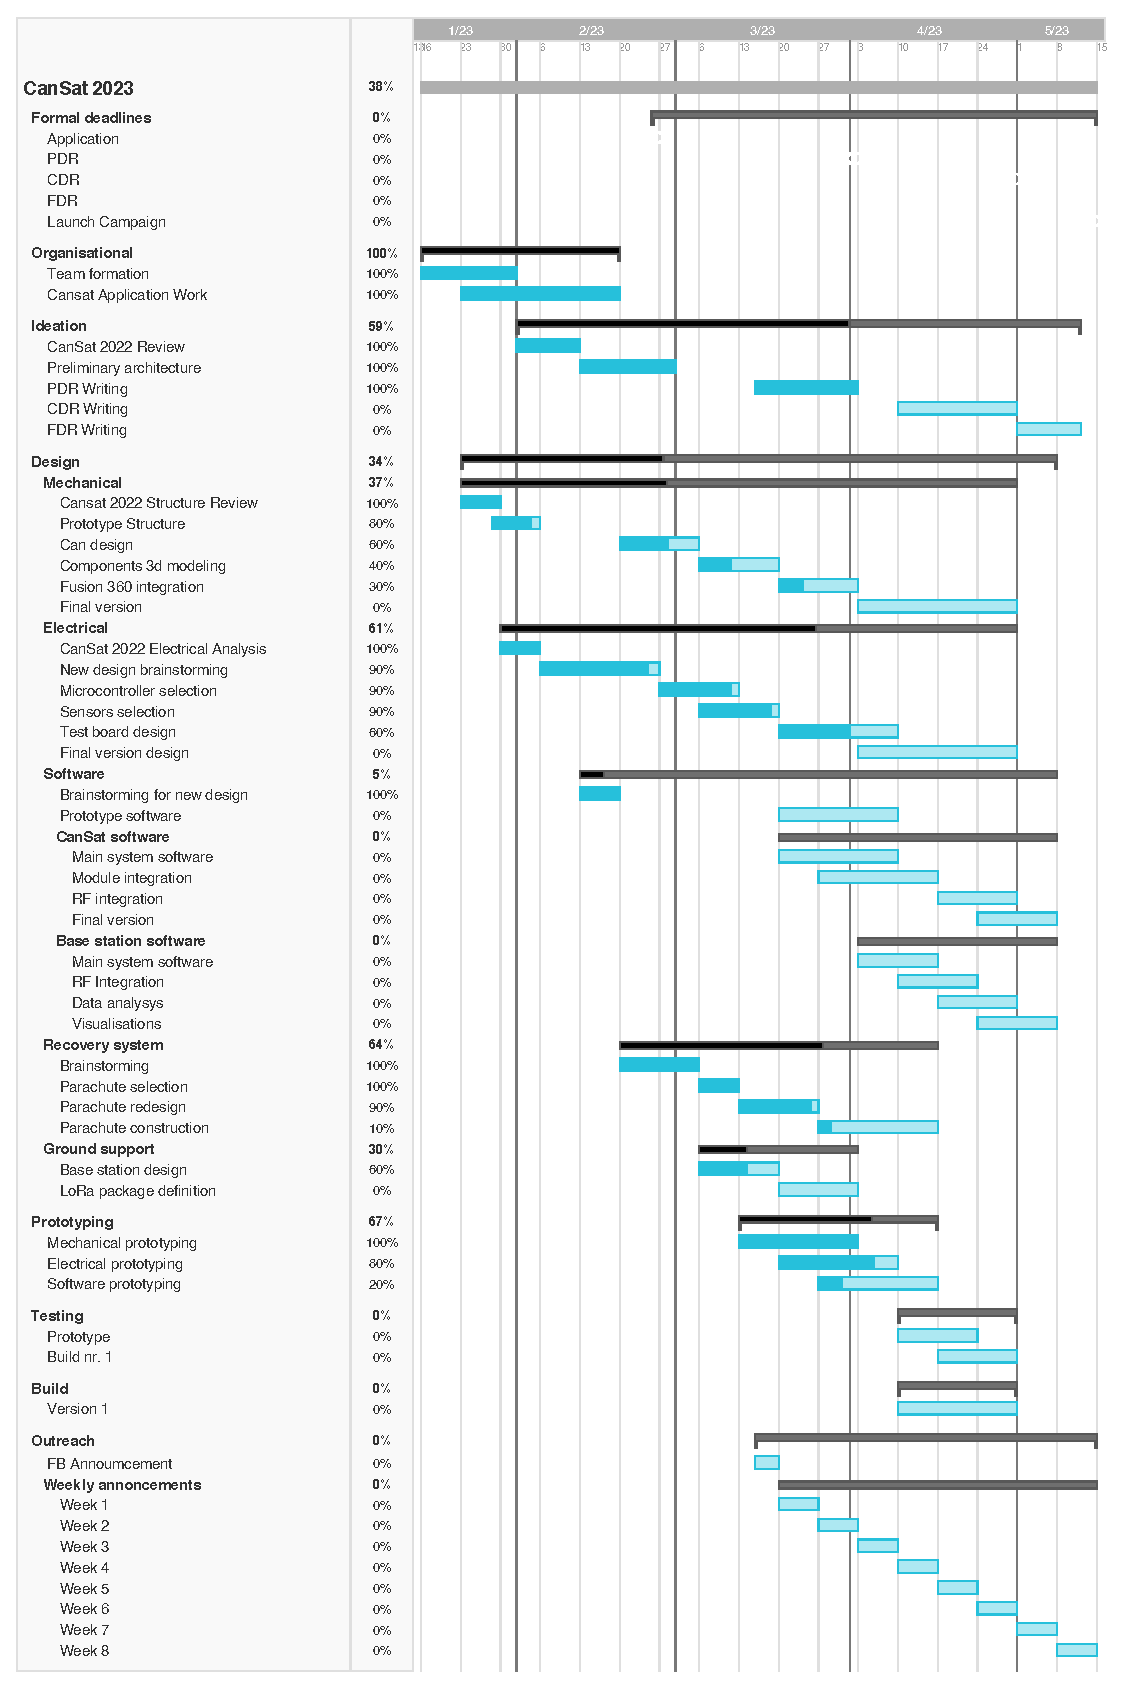
\includegraphics[width=13.5cm]{images/Gantt.eps}
%     %\caption{\small{CDOSR Gantt Chart for CanSat 2023.}}
%     \label{fig:gantt}
% \end{wrapfigure}


\begin{figure}[h]
    \centering
    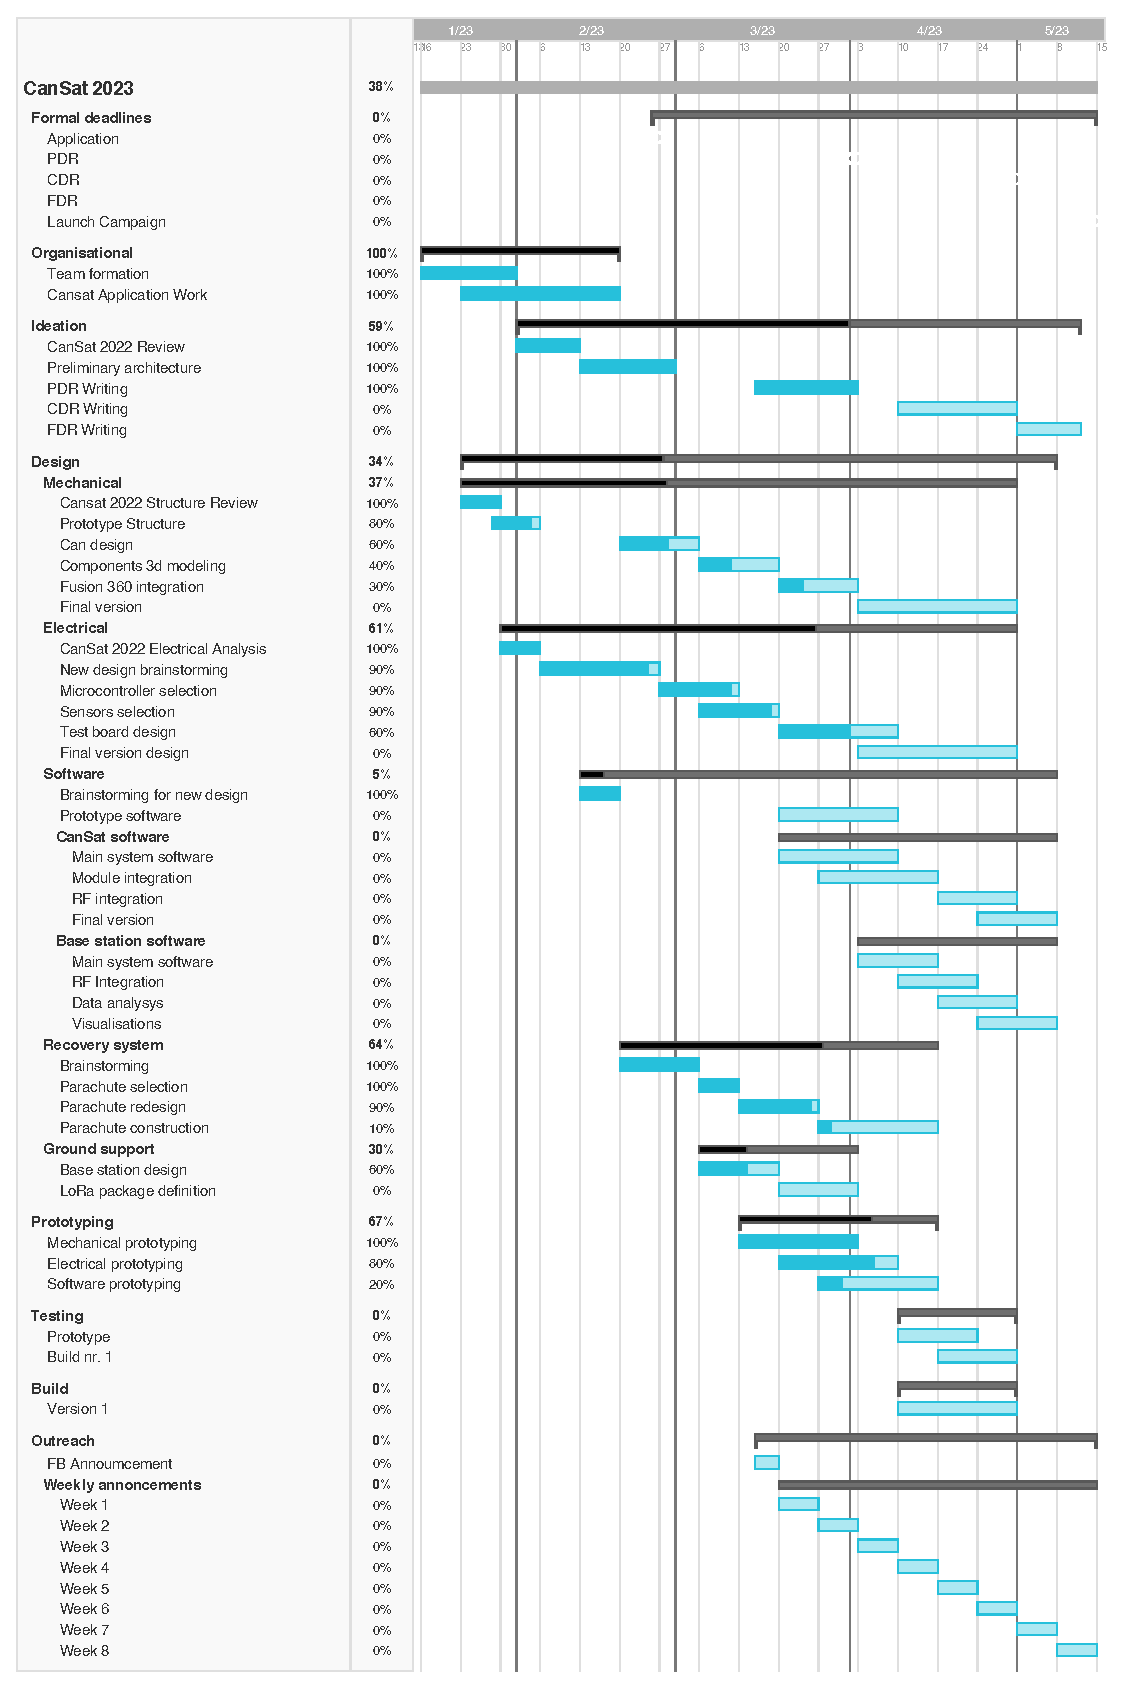
\includegraphics[width=11.7cm]{images/Gantt.eps}
    %\caption{\small{CDOSR Gantt Chart for CanSat 2023.}}
    \label{fig:gantt}
\end{figure}

% \begin{minipage}[c][\textheight]{\textwidth}
%     \vspace*{\fill}
%     \begin{figure}[h] % Use 'p' for a dedicated page for the figure
%     \centering
%     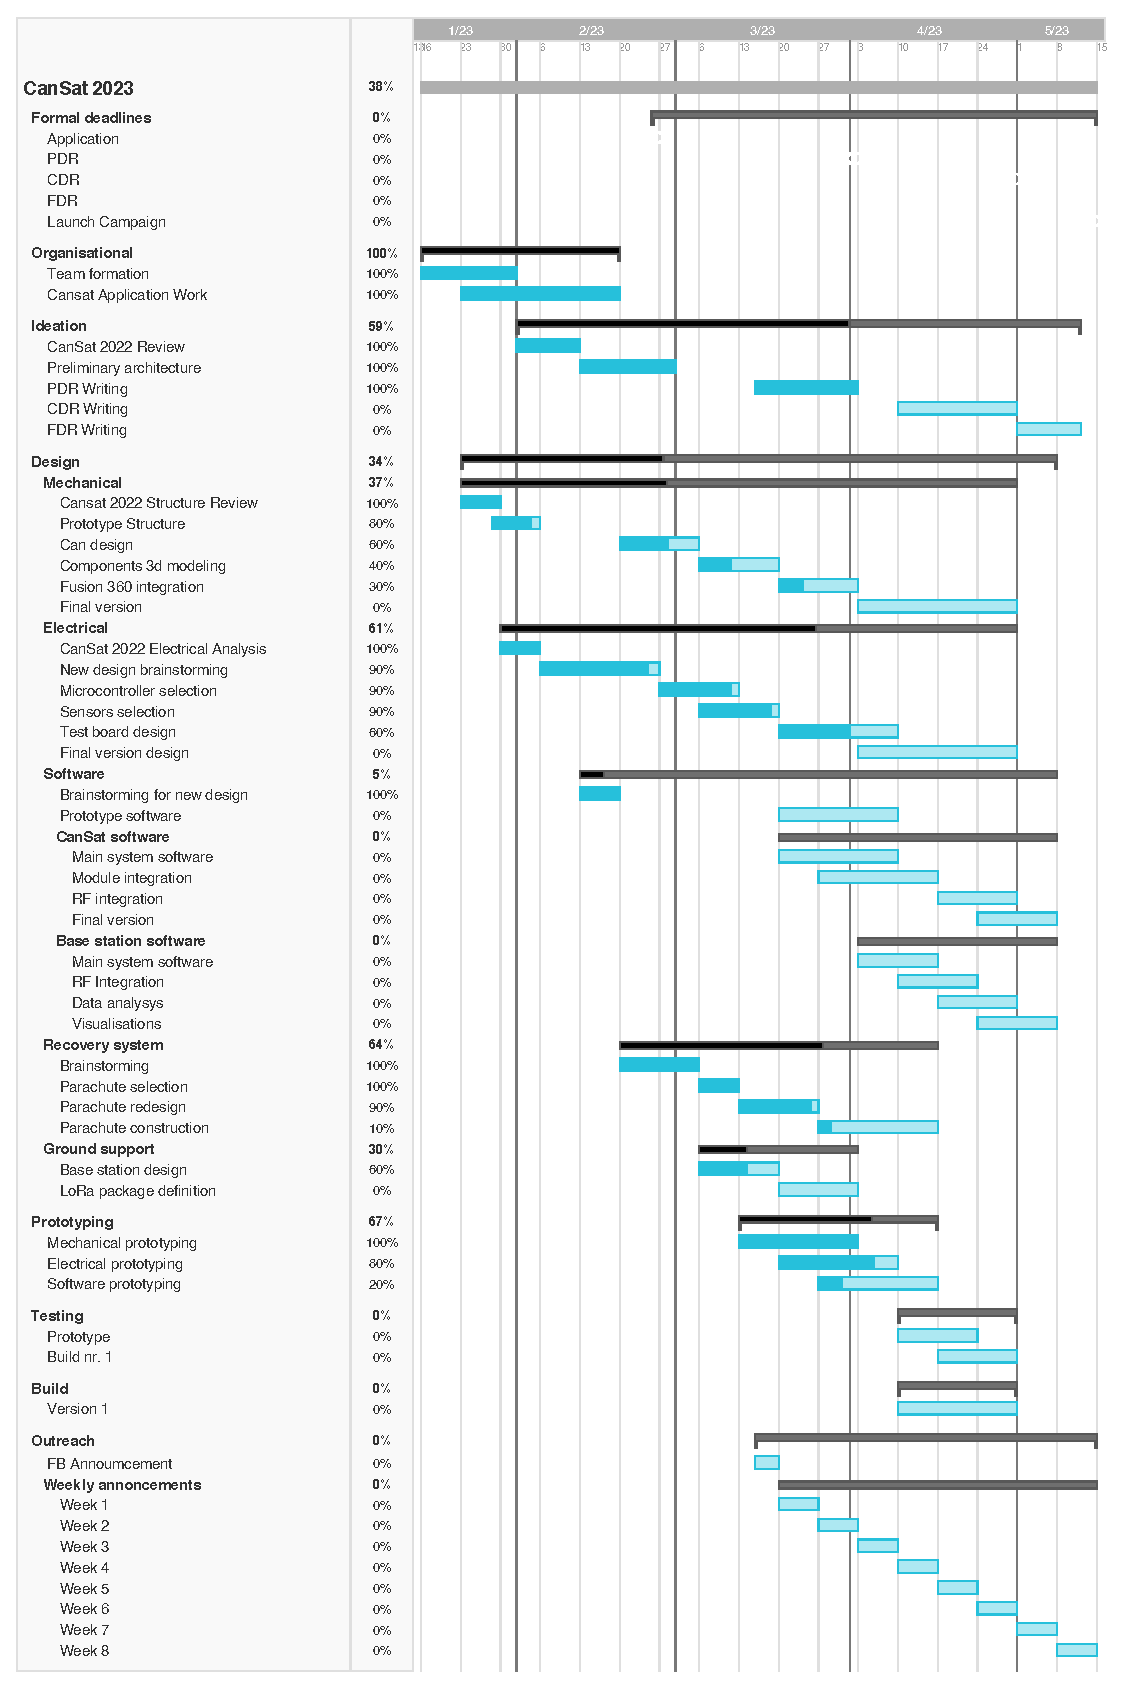
\includegraphics[width=\textwidth, keepaspectratio]{images/Gantt.eps}
%     %\caption{Your caption here}
%     \label{fig:gantt}
%     \end{figure}
%     \vspace*{\fill}
% \end{minipage}


\section{3D renderings}\label{A2}
\begin{wrapfigure}{l}{0.95\textheight}
    \centering
    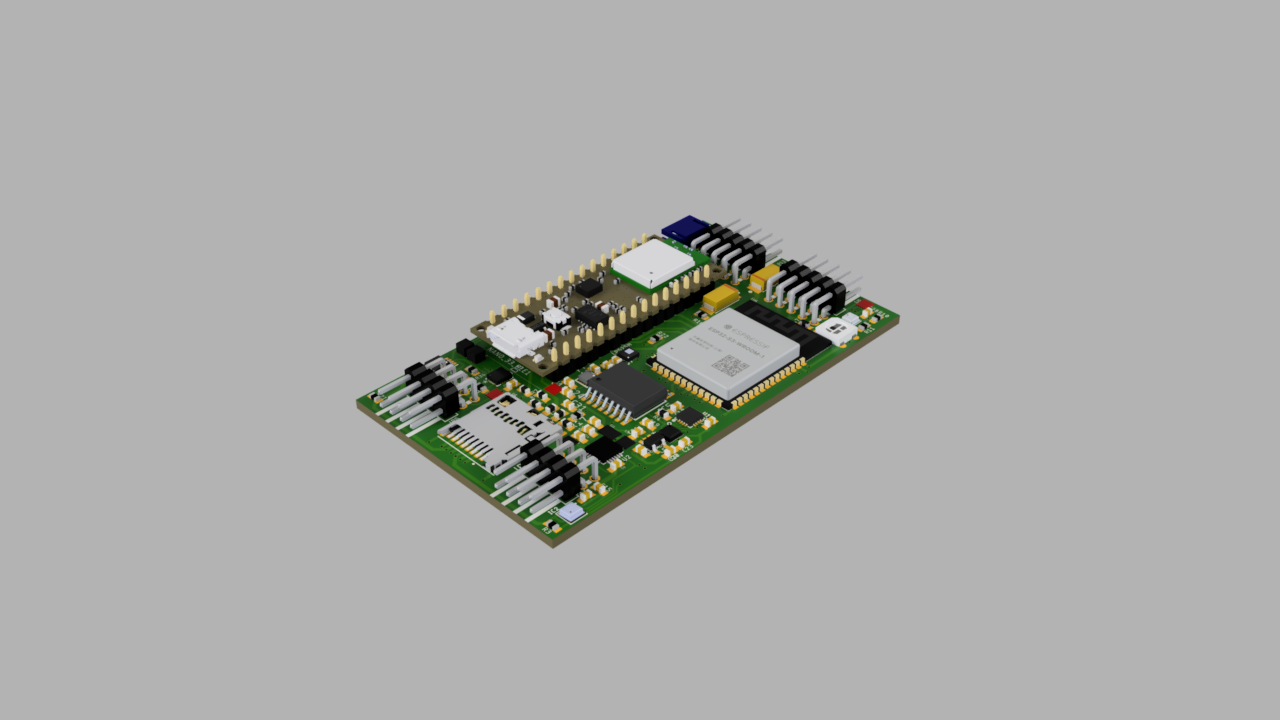
\includegraphics[width=11cm]{images/Sensor_board.png}
    %\caption{\small{CDOSR Gantt Chart for CanSat 2023.}}
    \label{fig:img1}
\end{wrapfigure}

\begin{wrapfigure}{l}{0.95\textheight}
    \centering
    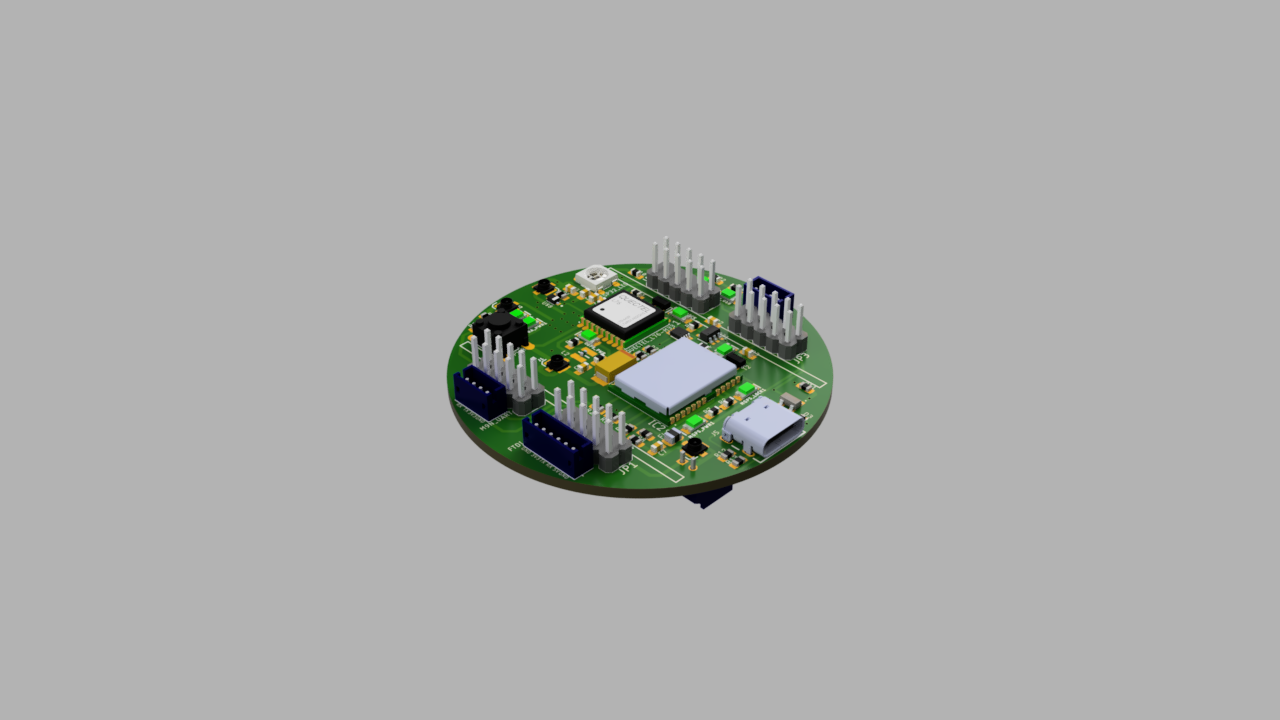
\includegraphics[width=11cm]{images/Topboard.png}
    %\caption{\small{CDOSR Gantt Chart for CanSat 2023.}}
    \label{fig:img2}
\end{wrapfigure}

\begin{wrapfigure}{l}{0.95\textheight}
    \centering
    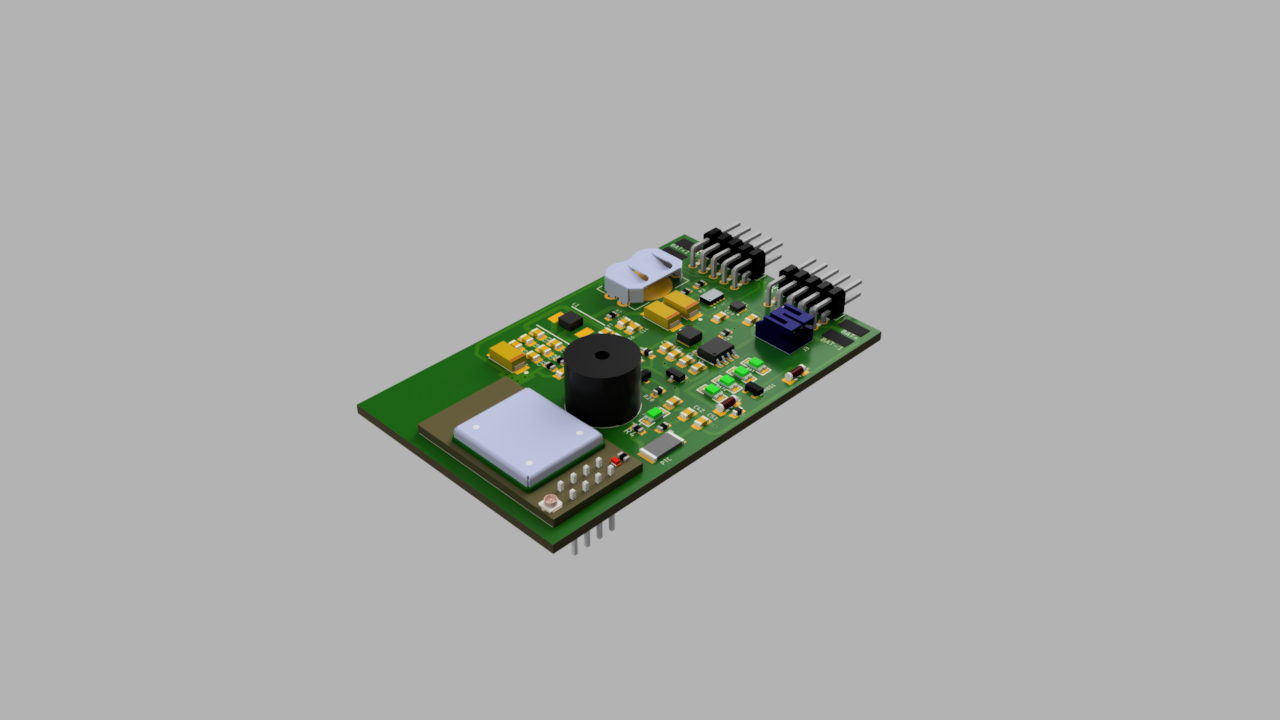
\includegraphics[width=11cm]{images/Power_board_v1.png}
    %\caption{\small{CDOSR Gantt Chart for CanSat 2023.}}
    \label{fig:img3}
\end{wrapfigure}

\begin{wrapfigure}{l}{0.95\textheight}
    \centering
    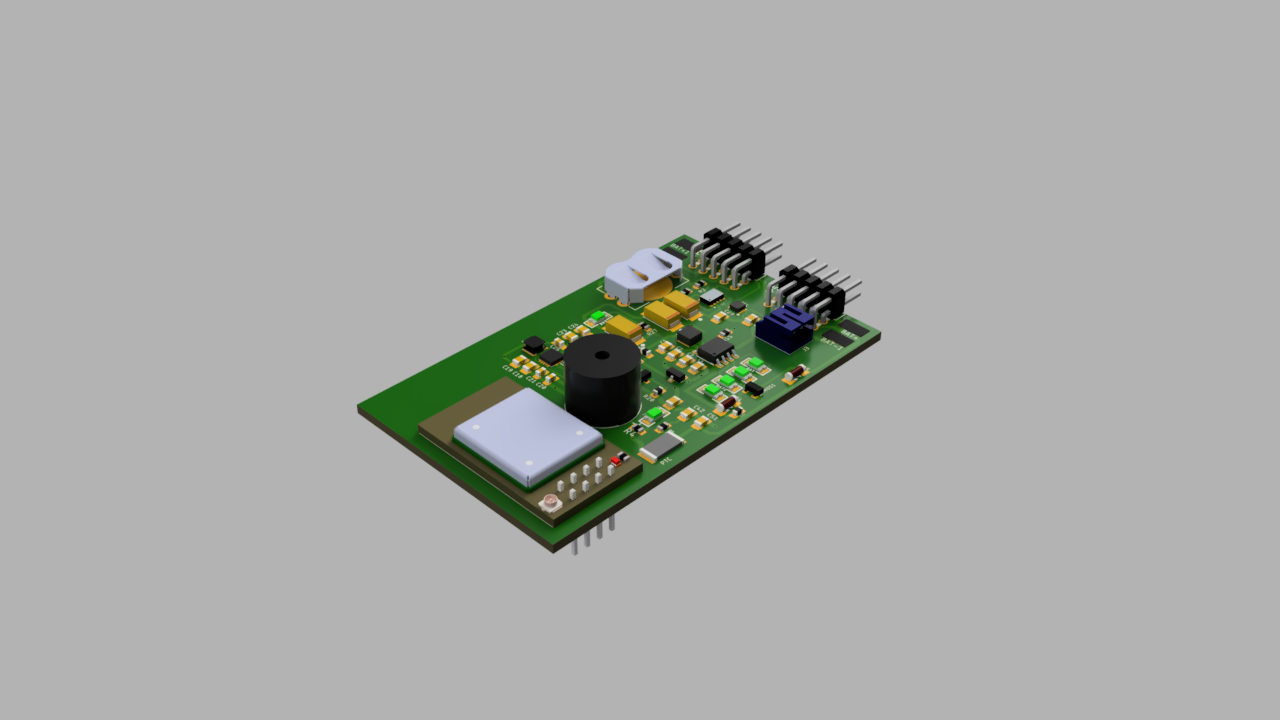
\includegraphics[width=11cm]{images/Powerboard_v2.png}
    %\caption{\small{CDOSR Gantt Chart for CanSat 2023.}}
    \label{fig:img4}
\end{wrapfigure}

\begin{wrapfigure}{l}{0.95\textheight}
    \centering
    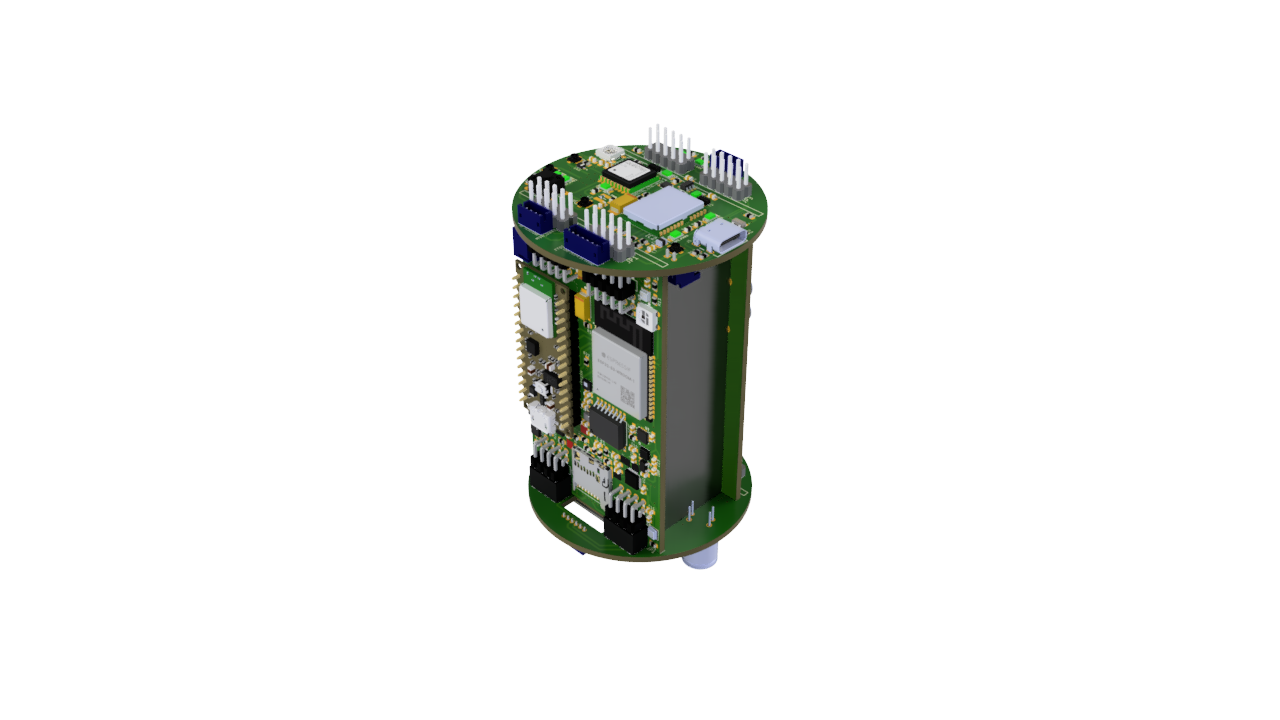
\includegraphics[width=11cm]{images/Assembled cansat.png}
    %\caption{\small{CDOSR Gantt Chart for CanSat 2023.}}
    \label{fig:img5}
\end{wrapfigure}

\section{PCB Schematics}\label{A3}
\end{document}

\end{document}
